The present chapter will give some general explanations on the physical processes that explain the observed sea state properties. It is now well understood that ocean waves derive most of their energy from the wind, and lose most of it to the ocean turbulence as they break. 
One particular motivation for understanding these physical processes is that beyond the wave spectrum, we may be able to quatify the fluxes of energy 
and momentum in and out of the wave field. 
Indeed, the generation of waves by the wind is thus associated to vertical fluxes of horizontal momentum and energy going 
from the wind to the wave field. This flux of momentum generally accounts for more than 70\% of the total momentum flux going 
from the atmosphere to the ocean, this total flux is usually called the wind stress. That air-sea momentum flux does not remain in the wave field, 
but rather it is lost by wave dissipation, mostly due to wave breaking, and ends up in the ocean currents. Most of this momentum 
loss happens at the same place where waves were generated: the wave field is thus largely 'transparent' to this momentum flux. However, a few percent of this 
momentum flux propagates away across ocean basins and is transformed into changes in sea level -- this is known as wave set up -- and currents on the beaches where waves break. 
These currents are the longshore currents. This transformation of wave momentum in the nearshore is the topic of chapter \ref{ch_littoral}. 
%%%%%%%%%%%%% figure
\begin{figure}[hbt]
\centerline{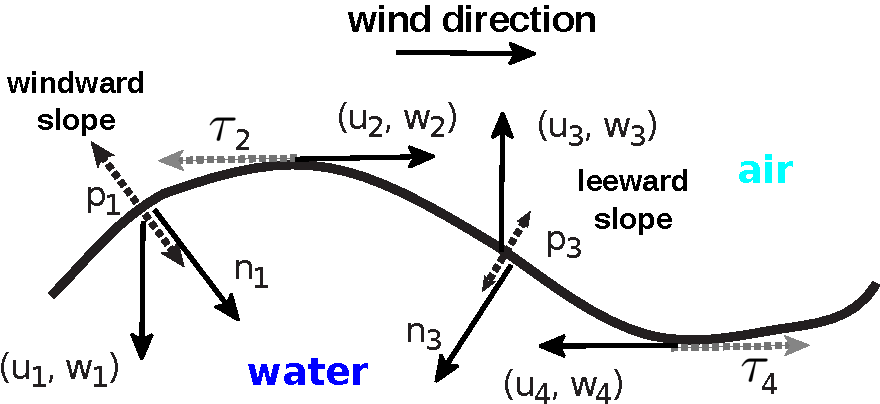
\includegraphics[width=0.7\textwidth]{FIGS_CH_SOURCETERMS/air_sea_fluxes_en.pdf}}
%\vspace{3.64in}
  \caption{Fluxes at the air-sea interface, at four phases of the wave profile: 1 windward slope, 2 crest, 3 leeward slope, 4 trough. 
The energy flux from the atmosphere to the ocean is the work of the stresses acting on the sea surface, 
   $\left[p \mathbf{n} + \tau\right] \bcdot (u,w)$, with $\mathbf{n}$ the unit normal vector pointing to the water side.
   As a result, if the air pressure is higher on the windward slope, then 
   $p_1 w_1 \left.\frac{\partial \zeta}{\partial x}\right|_1 > p_3 w_3 \left.\frac{\partial \zeta}{\partial x}\right|_3$
   and the pressure-related flux is positive towards the water side. 
   Likewise, if the shear stress  $\tau$ is opposed to the velocity vector (as here), the flux $\tau u$ induced by shear stresses is 
negative (i.e. energy goes from the water to the air). Similarly, the momentum flux is the average 
stress acting on the surface. Because of the surface slope, the vertical flux of horizontal momentum is the 
average of  $p {\partial \zeta}/{\partial x}$ plus the average of  $\tau_x$.} \label{airseaflux}
\end{figure}
%%%%%%%%%%%%% end of figure
%We shall see also in the next chapter that waves also carry some horizontal momentum, which, for monochromatic waves 
%of phase speed $C$ has a density per unit horizontal surface equal to $\rho_w g E/C$ and points in the wave propagation direction. 


Besides the generation or attenuation by the wind and dissipation associated to breaking, a third mechanism is very important for the 
evolution of the waves in deep water. It is the non-linear evolution of the waves which can be understood as a wave-wave scattering process: waves components 
exange energy and momentum, some components grow and others decay. In order to make things simple, we will now consider separately each of these three processes. 

\section{Generation of waves by the wind}
The fraction of the wave energy that is in the water is $(\rho_w -\rho_a)/\rho_w \simeq 99.9$\%. Hence the transfer energy from wind to waves 
involves a flux of energy through the sea surface. Because the surface is a material surface, this flux cannot happen by advection, it thus requires the 
work of stresses on the surface, either the tangential stresses $\tau$ or the normal stresses, i.e. the pressure $p$. In the case of tangential stresses, 
the work is the correlation of 
the along-surface shear stress with the along-surface orbital velocity. The work of normal stresses is the correlation of pressure times the velocity normal to the surface
 (see figure \ref{airseaflux}). A quantification of these energy fluxes thus require the identification of processes that produce pressure and shear stresses on the surface. 
The first hypotheses on wave generation followed the theory of hydrodynamic instabilities. The air flow over a water surface is a particular case of a sheared flow in a stratified 
medium that may lead to the Kelvin-Helmholtz (KH) instability. This may indeed be important for very high winds speeds \citep{Soloviev&al.2014}, but it cannot explain the 
initial growth of waves under moderate winds. In particular, KH theory predicts instabilities for an air-water interface for wind speeds above 6.5 m~s$^{-1}$ (Jeffreys 1925), 
but ripples already appear on the water surface for winds as low as  $U= 1.1$~m~s$^{-1}$
(Kahma et Donelan 1988\nocite{Kahma&Donelan1988}). 

This initial growth of ripples is rather well explained by the effect of turbulence in the air advected by the wind \cite{Phillips1957}. 
That process is very soon overtaken by the feedback caused by the wave-induced pressure oscillations in the air, as the airflow is modified by the presence of waves. 
 When waves travel slower than the wind projected in their propagation direction, the pressure is slightly higher on the windward face, typically of the order of a few Pascals,
and lower on the leeward side. 


We are thus going to generalize the Airy wave theory of chapter \ref{ch1b}. To simplify the calculations we will replace the wave amplitude $a$ by a complex amplitude  $Z_0=a \er^{\ir \Theta_0}$, so that the sea surface elevation is 
\begin{equation}
    \zeta= \overline{\zeta} + \Re \left[ Z_0 \mathrm{e}^{\mathrm{i}{\mathbf k}\bcdot{\mathbf x} - \sigma t} \right],\label{polzetain}
\end{equation}
where we recall that $ \Re$ represents the real part of a complex number. In a first approximation, we will assume that the atmospheric pressure is proportional but shifted in phase compared to the amplitude of the surface elevation, 
\begin{equation}
 p_a= \overline{p}_a + \rho_w g \Re \left[ \left( \alpha + {\mathrm i}\beta\right)   Z_0 \mathrm{e}^{\mathrm{i}{\mathbf k}\bcdot{\mathbf x} - \sigma t} \right], \label{wave_induced_pa}
\end{equation}
where $\alpha$ represents the in-phase oscillations and $\beta$ the oscillations in quadrature. 

Here we will take $\alpha=0$ for simplicity as we shall see that it is not important for wind-wave growth. 
When $\beta \ll 1$, we assume that the air pressure only makes a small $O(\beta)$ correction to the solution we found in  chapter \ref{ch1b}. 
Bernoulli's eq. (\ref{p_all}) at the surface now has a forcing term from the atmospheric pressure. For propagating waves we can neglect $\gamma(t)$, giving, 
\begin{equation}
    \frac{\partial \phi}{\partial t} \simeq 
       - g \zeta - \overline{p}_a/\rho_w  - g \Re \left[{\mathrm i}\beta   Z_0 \mathrm{e}^{\mathrm{i}{\mathbf k}\bcdot{\mathbf x} - \sigma t} \right].\label{Bernoulli_linin}
\end{equation}

Taking  $\partial (\ref{Bernoulli_linin} \textrm{~at z=}\zeta)/\partial t $
+$g\times$(\ref{surface_lin}) we eliminate the unknown $\zeta$. 
\begin{equation}
  \frac{\partial^2{\phi}}{\partial{t^2}}+g\frac{\partial\phi}{\partial z} + g \sigma \beta   \Re \left[   Z_0 \mathrm{e}^{\mathrm{i}{\mathbf k}\bcdot{\mathbf x} - \sigma t} \right] =0, \quad \mbox{at}
\quad  z=\overline{\zeta}. \label{surface 1in}
\end{equation}
Since the last term is already of order $\beta$, we can use the Airy theory result that is valid at order 0: eq. (\ref{afromPhi0}) gives   $Z_0={\mathrm i}{\sigma}\Phi_{0}/g$, and we recall that Laplace equation and the bottom boundary condition gives us 
\begin{equation}
    \phi=\Re \left( \Phi_0
    \frac{\cosh\left(kz+kh\right)}{\cosh\left(kD\right)}
     \mathrm{e}^{\mathrm{i}{\mathbf k}\bcdot{\mathbf x} - \sigma t} \right),
    \label{phi1recall}
\end{equation}.

 We can thus re-write eq. (\ref{surface 1in}) in terms of the surface complex amplitude $\Phi_0$,
\begin{equation}
    -\sigma^2 + g k \tanh (kD)+\ir \beta \sigma^2 =0.\label{disp_in}
\end{equation}
We thus have an order $\beta$ correction to the dispersion relation, namely the frequency now has an imaginary part.  At first order in $\beta$, this is 
\begin{equation}
    \sigma= \left(1+\frac{\ir \beta}{2}\right)\sqrt{g k \tanh (kD)},\label{disp_in}
\end{equation}
and  this gives an exponential growth if $\beta > 0$,   or decay term  if $\beta < 0$, 
\begin{equation}
    \zeta= \overline{\zeta} + \Re \left[ Z_0 \mathrm{e}^{\beta \sqrt{g k \tanh (kD)}  t/2}  \mathrm{e}^{\mathrm{i}{\mathbf k}\bcdot{\mathbf x} - \sqrt{g k \tanh (kD)}  t} \right].
\end{equation}
From a physical point of view it is more natural to keep our dispersion relation be redefining $\sigma=\sqrt{g k \tanh (kD)}$ and redefining the amplitude as slowly varying in time
\begin{equation}
a(t)= a \mathrm{e}^{\beta \sigma t/2} 
\end{equation}

With these notations, the phase is the same as in chapter 2, $\Theta = {\mathbf k}\bcdot{\mathbf x} - \sigma t + \Theta_0$, and  the full solution to first order in $\beta$ is
\begin{eqnarray}
    \zeta-\overline{\zeta}&=&   a(t) \cos \Theta - \beta \frac{a(t)}{2}  \sin \Theta, \\
    \phi &=& \frac{g a(t)}{\sigma} F_{CC} \sin \Theta + \beta g \frac{a(t)}{2 \sigma}  F_{CC}  \cos \Theta , \label{phi_in} \\
    \xi_3 &=&  a(t)  F_{SS} \cos \Theta - \beta \frac{a(t)}{2}  F_{SS}  \sin \Theta , \label{phi_in} \\
    p-\overline{p}^H &=&   \rho_w g a(t) F_{CC} \cos \psi -\rho_w g \beta  \frac{a(t)}{2}  F_{CC} \sin\Theta, \\
    \frac{{\mathrm d} a(t)}{{\mathrm d} t}&=&\frac{\beta \sigma a(t)}{2}, \\
    \frac{{\mathrm d}}{{\mathrm d} t}\frac{a^2(t)}{2} &=&\beta \sigma
    \frac{a^2(t)}{2}  \quad \mathrm{giving} \quad \frac{{\mathrm d} E}{{\mathrm d} t}= \sigma \beta  E  \label{eq:energy_wind_growth}
\end{eqnarray}
where $F_{CC}=\cosh(kz+kh)/\cosh(kD)$ and $F_{SS}=\sinh(kz+kh)/\sinh(kD)$. For those alergic to complex frequencies, the same solution is obtained by allowing the amplitudes to evolve slowly in time from the beginning of the derivation, keeping track of the two time scales, slow for amplitude evolution and fast for phase evolution. That method requires a careful book-keeping of the different terms that come from the time derivative. For example, 
\begin{equation}
   \frac{\partial \phi}{\partial t} = - g a(t) F_{CC} \cos \Theta + \beta g \frac{a(t)}{2}  F_{CC}  \sin
    \Theta  + \beta g \frac{a(t)}{2 }  F_{CC}  \sin \Theta -  \beta^2 g \frac{a(t)}{4}  F_{CC}  \cos \Theta,
\end{equation}
with the first two terms coming from the phase of eq. (\ref{phi_in}), and the amplitude evolution giving the last two terms. We can see that at order $\beta$ we neglect the last $O(\beta^2)$ term and this is a solution to eq. (\ref{Bernoulli_linin}). 


It is an interesting exercise to also compute the Eulerian-mean flux of momentum at each depth,  $\langle u w \rangle$, and prove that 
it is still zero at order $\beta$. The Lagrangian flux of momentum is given by the mean pressure acting on the material surfaces, i.e. $ p \partial \xi_3/\partial x$  for the $x$-component of the momentum. That Lagrangian flux has the same profile as the Stokes drift, given in the next chapter. This means that when the wind generates waves, the (Lagrangian) wave momentum increases in the water column \citep{Ardhuin&al.2008b}. 

%In the absence of other processes, this surface pressure yields an exponential growth or decay of the wave energy, depending on the sign of $\beta$. 


\subsection{Measuring and parameterizing wind-wave generation}
With an air pressure that is proportional to the surface elevation, the 
 energy growth in eq. (\ref{eq:energy_wind_growth}) can be written as a source term  
\begin{equation}
    S_{\mathrm{in}}\left(f,\theta\right)=\sigma \beta E\left(f,\theta\right).
\end{equation}
The magnitude of the non-dimensional growth rate $\beta$ is a key parameter 
to determine the energy balance with dissipative and non-linear processes, and, as a result, the shape of the wave spectrum. 
Numerical wave models all use semi-empirical parameterized expressions, with  $\beta$ a function of the relative direction between the wind and the waves, and a function
of the ratio of the wind speed and the phase speed. 

In most model parameterizations,   $\beta$ is inspired from theoretical results \citep[e.g.][]{Miles1959,Fabrikant1976,Miles1996b}, 
with empirical adjustments to the few 	available measurements of pressure over waves, or numerical simulations of air flow over waves, 
or observed wave groth \citep{Plant1982}, or measurements of pressure-slope correlations \citep{Snyder&al.1981,Donelan&al.2005b,Donelan&al.2006}.

\subsection{Parameterizations based on observations}
\cite{Snyder&al.1981} performed an important field experiment in the bight of Abaco, in the Bahamas, in order to 
reconcile the previous diverging observations by \cite{Dobson1971} and \cite{Snyder&Cox1966}. Their measurements performed under light to moderate 
wind speeds are summarized by a growth rate
\begin{equation}
    \beta=\max\left\{0,0.25 \frac{\rho_a}{\rho_w}\left[28\frac{u_\star}{C}
    \cos\left(\theta_\star - \theta\right)-1\right]\right\}.\label{Snyder}
\end{equation}
where $C$ is the phase speed $\rho_a$ and $\rho_w$ are the densities of air and water, and $u_\star=\left<u'w'\right>^{1/2}=\sqrt{\tau_a / \rho_a}$ where $\tau_a$ is the 
air-sea momentum flux per unit horizontal surface, usually called `wind stress'. 
This parameterization is used in the `Cycle 3' of the WAM model \citep{WAMDI1988}. 

The measurements by \cite{Snyder&al.1981} have been confirmed by other experiments, for example in the North Sea by \cite{Hasselmann&Bosenberg1991}. 
Unfortunately these measurements at sea are made only with moderate wave heights and wind speed, and only for waves around the spectral peak. 

Besides, most wind measurements at sea consist of mean wind speed and direction at a fixed height, typically 5~m, without the 
rapid fluctuations needed to estimate the friction velocity $u_\star$. A link between this wind speed and the wind stress is provided 
by assuming that the turbulent momentum flux 
$\left<u'w'\right>$ is constant with height (which is not so true near the surface in the presence of waves), and that the mixing can be parametrized 
by an eddy viscosity of the form $\nu_T=l^2
\partial U/\partial z$ where the mixing length is given by $l=\kappa z$
with  von K{\'a}rm{\'a}n's constant $\kappa=0.41$. Under these assumptions, the wind speed profile is a logarithmic as a function of height, 
\begin{equation}
    U\left(z\right)=\frac{u_\star}{\kappa}\ln \left(z/z_0\right),
\end{equation}
starting from $0$ at the roughness height $z_0$. There are many discussions on the proper way to estimate $z_0$, but a first reasonable 
guess is provided by the dimensional analysis of  \cite{Charnock1955}, 
\begin{equation}
    z_0\simeq\alpha_{CH} u_\star ^2/g,
\end{equation}
where $\alpha_{CH} \simeq 0.015$ is Charnock's 'constant'. 

From this type of expression, several adjustement have been proposed, in particular it appears that 
the Charnock coefficient may vary with wave age, with an increase for young waves. This is how  \cite{Janssen1991} parameterized 
the numerical results of a coupled wave-atmosphere boundary layer model. 

For very young waves,  with $U_{10}/C_p > 3$ there are also clear signs of strong air flow detachment from the sea surface, which 
leads to an increase of $\beta$ and decrease for extremely young waves when the air flow is fully detached \citep{Donelan&al.2006,Babanin&al.2007}. 
This detachement of the air flow and attenuation of the short waves by the wind \citep{Soloviev&al.2014} are possible explanations, together with the effect of 
sea spray \citep{Andreas2004}, for the reduction of the drag coefficient $C_d = u_\star^2 / U_{10}^2$ in hurricane conditions. This is a very active topic of research 
with important consequences for the understanding and forecasting of extreme storm surges \citep[e.g.][]{Resio&Westerink2008}. 


\subsection{Short waves and multiple-scale interactions}
For the high frequency part of the spectrum, say $f> 3f_p$, there are no direct measurements of the pressure-slope correlations. The growth parameterizations 
are thus inferred from the observation of wind-wave growth \citep[e.g.][]{Plant1982}, and numerical simulations 
that are consistent with an energy source term $S_{\mathrm{in}}$ proportional to $u_\star^2 \cos^2
\left(\theta_\star - \theta\right)$. Besides, approaching the sea surface from above, a growing fraction of the momentum flux is carried by the wave orbital motion, in the 
form of a correlation $\overline{u w}$. A likely consequence is that the short waves, which are affected by the air layers closest to the 
surface, only feel a reduced wind stress as they are 'sheltered' by the longer waves  \citep{Hara&Belcher2002}.
In the presence of long waves, we thus expect that the growth rate of shorter waves is strongly reduced. 
%%%%%%%%%%%%% figure
\begin{figure}
\centerline{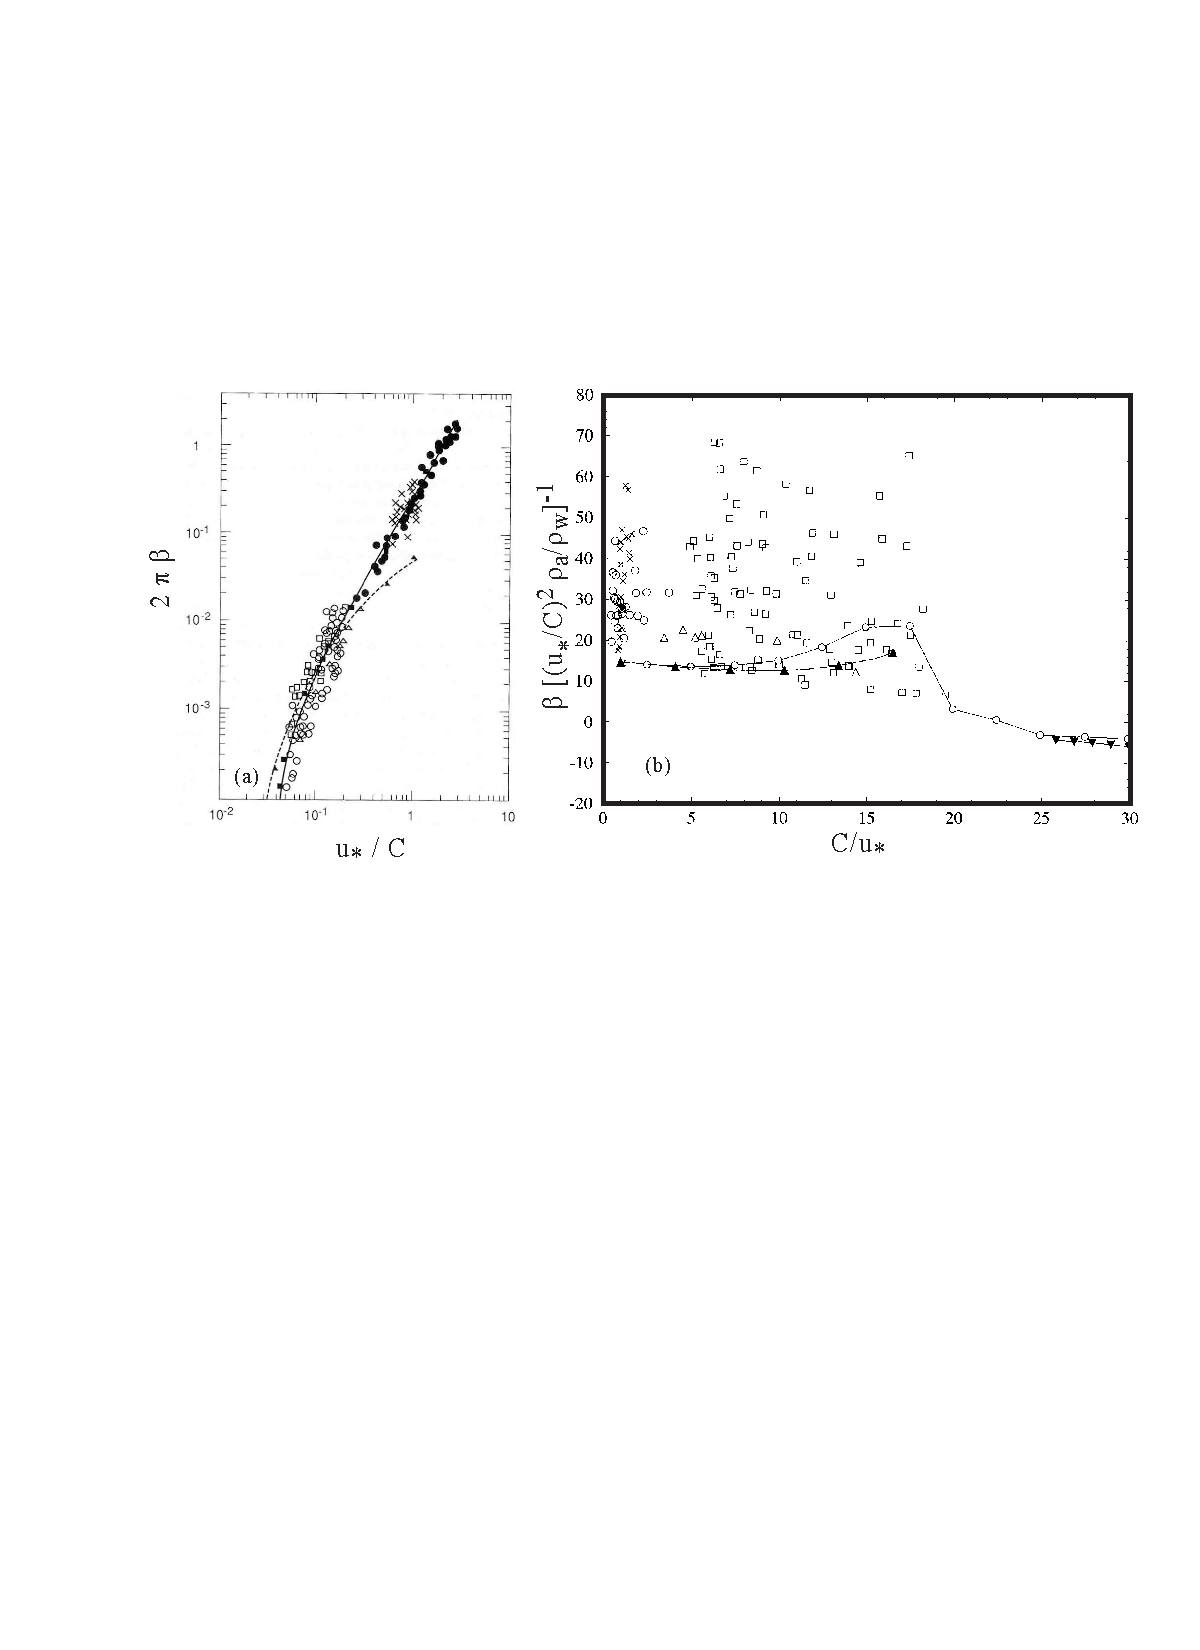
\includegraphics[width=\textwidth]{FIGS_CH_SOURCETERMS/Belcher_EJMB1999.pdf}}
%\vspace{3.64in}
\caption{Growth rate of waves propagating in the wind direction, combining observations and theory.}{a. solid line: Miles theory 
as extended by Fabrikant and Janssen, dashed:
measurements of \cite{Snyder&al.1981} as summarized by eq. (\ref{Snyder}), symbols: estimations compiled by Plant (1982), this figure 
is taken from \cite{Janssen&al.1994}. (b) growth rate for a non-dimensional wavenumber  $k z_0=10^{-4}$ (filled triangles) compared
to numerical model results with connected circles by \cite{Mastenbroek1996}  and the \cite{Plant1982} data (other symbols), that figure is 
taken from \cite{Belcher1999}.} \label{fig_Belcher}
\end{figure}





\subsection{In summary}
Wind is a source of energy  ($S_{\mathrm{in}} > 0$) for all spectral components 
such that  $U/(C \cos \theta_u - \theta) > 1$. 
In the spectral plane, this corresponds to a region bounded by the straight line defined by $U/(C \cos \theta_u - \theta) = 1$. 
The other components, with $U/(C \cos \theta_u - \theta) < 1$ are a sink of energy for the waves  ($S_{out} < 0$), and thus a source of energy for the wind. 

The source term that represents the interaction between the atmosphere and the waves can be written as 
\begin{equation}
S_{\mathrm{atm}}(k,\theta)=S_{\mathrm{in}}(k,\theta)+S_{\mathrm{out}}(k,\theta) = \sigma \beta E(k,\theta),
\end{equation}
where the non-dimensiona growth parameter $\beta$ is of the order of $30 \rho_a u_\star / C / \rho_w$ for $1 < U/(C \cos \theta_u - \theta) < 3$, 
and a much smaller negative number, typically $-2 \times 10^{-6}$ for  $U/(C \cos \theta_u - \theta) < 1$. This negative 
part appears to be non-linear with a magnitude of $\beta$ that increases with the steepness of the swell. 

In general it is expected that the growth rate of one component is also a function of the amplitude of other components, but that effect is very poorly 
known.

\section{Weakly non-linear evolution}
Because waves are not exactly linear, 
they produce many interesting effects: presence of harmonics, recurrence patterns, instabilities ... that are further discussed in Part 3. Here we will focus on the evolution of the wave spectrum that comes from the exchange of 
energy between different spectral components. 

This spectral evolution is generally described as a wave-wave interaction process, which is a particular case of wave scattering. In the case of a continuous 
spectrum, this effect is also known as `weak turbulence', as it exhibits Kolmogorov-type solutions with a cascade of energy towards the short waves as well as an 
inverse cascade towards the longer waves. The rate of change 
of the spectrum due to this non-linear effect was determined by Klaus
Hasselmann (1960\nocite{Hasselmann1960},1962\nocite{Hasselmann1962}) and Vladimir Zakharov
(1968\nocite{Zakharov1968}), starting from the Euler equations and assuming a quasi-Gaussian sea state, and looking for the large time limit. These two publications used different methods that are equivalent, as shown by \citet[e.g.][]{Elfouhaily&al.2000} and \citet[e.g.][]{Resio&al.2001}.
The confirmation of this theory using more complete equations of motions is fairly recent \citep{Tanaka2001b,Korotkevich&al.2008}. 
The experimental verification in the case of a pair of monochromatic wave train was first performed by \cite{McGoldrick&al.1966}, who showed that two wave trains of different 
frequencies and directions can create a third wave train with yet another frequency and direction. 

Hence, within the wave spectrum, there is a continuous exchange of energy between components that strongly modifies the shape of the spectrum. This exchange is 
strongest for steep waves. The only remaining doubts about this theory are its applicability to shallow water or in cases with strong horizontal variations of depth or currents on the scale of the wavelength. In the latter case one cannot take the large time limit and the interactions are generalized to include near-resonances \citep{Stiassnie2004,Annenkov&Shrira2006}.




\subsection{Wave-wave interation theory}
When solving the Euler equations, we can keep the non-linear terms that were discarded by Airy, 
and write the solution as an expansion in powers of the wave slope $\varepsilon = k a $.  One then finds a first order solution that is a superposition of Airy waves
\begin{equation}
 \zeta_1=\sum_{\kb,s} Z(\kb,s) \er^{\ir \left[\kb \bcdot \xb -s \sigma t\right]}
\end{equation}
and that can be introduced into the second order equations. 

In order to make things more simple, let us imagine that the full boundary condition is given by, 
\begin{equation}
\left[ \frac{\partial }{\partial t^2} - g k \tanh(kD) \right]\zeta  = g \bnabla \zeta \bcdot \bnabla \zeta.
\end{equation}
At second order this gives the following forced harmonic oscillator equation 
\begin{equation}
\left[ \frac{\partial }{\partial t^2} - g k \tanh(kD) \right]\zeta_2  = g \bnabla \zeta_1 \bcdot \bnabla \zeta_1.
\end{equation}
If there are components $(\kb,\sigma)$ such that $\kb=\kb_1+\kb_2$ et $\sigma=\sigma_1+\sigma_2$ then the solution contain resonances. \cite{Phillips1960} showed
that such components do not exist because the dispersion relation of gravity waves does not have an inflexion point, hence there is no resonance at second order 
and the solution is bounded with a simple expression of the second order amplitudes as a function of the first order amplitudes, 
\begin{equation}
 \zeta_2=\sum_{\kb_1,s_1} \sum_{\kb_2,s} A (\kb_1,\kb_2,s_1,s_2) Z(\kb_1,s_1)  Z(\kb_2,s_2)  
\er^{\ir \left[(\kb_1 + \kb_2) \bcdot \xb -(s_1 \sigma_1+s_2 \sigma_2) t\right]} \label{zeta2}
\end{equation}
with $A (\kb_1,\kb_2,s_1,s_2)$ a constant coefficient given by
\begin{equation}
 A=\frac{\kb_1 \bcdot \kb_2 }{s_1 \sigma_1 s_2 \sigma_2 - g k \tanh(kD)}\label{eq:nl_A_simple}.
\end{equation}

The actual Euler equation (see Part 3) has a few extra terms but it is the same principle with a similar result, only expression for  $A$ is more complex. 
This second order elevation is the generalization of the first harmonic of a monochromatic waves: if the first order only contains waves of frequency $f$, 
the the second order has components with frequency $2f$ and 0. 

Things get more exciting when resonances exist. Resonances at second order exist for 
dispersion relation with an inflexion point, which is the case of gravity-capillarity waves or in the presence of sea ice, 
but we will not discuss this here. 
For gravity waves \cite{Phillips1960} showed that resonanced occur at third order. 
The third order amplitude is a solution of  a forced oscillator equation,
\begin{eqnarray}
\left[ \frac{\partial }{\partial t^2} - g k_4 \tanh(k_4 D) \right] Z_3(\kb_4)   = \sum_{k_1,k_2,k_3,s_1,s_2,s_3} & &B(\kb_1,\kb_2,\kb_3,s_1,s_2,s_3) Z(\kb_1,s_1)  Z(\kb_2,s_2)  
 Z(\kb_3,s_3)  \nonumber \\
& &\er^{\ir \left[(\kb_1 + \kb_2 + \kb_3) \bcdot \xb -(s_1 \sigma_1+s_2 \sigma_2 + s_2 \sigma_3) t\right]}
\end{eqnarray}
in which $\kb_3=\kb_4-\kb_1-\kb_2$. The right hand side is resonant for 
$\kb_4=\kb_1+\kb_2+\kb_3$ and $\sigma\left(k_4\right)=\sigma_1+\sigma_2-\sigma_3$. This resonance condition is satisfied for an inifinite 
number of quadruplets ($\kb_1$, $\kb_2$, $\kb_3$, $\kb_4$), as illustrated in figure \ref{fig_DIA} for the case of deep water. Resonances 
also exist in shallow water, only the shape of the curves are changed. 

%%%%%%%%%%%%%%%%%%%%%%%%%%%%%%%%%%%%%%%%%%%%%%%%%%%%%%%%%%%%%%%%% figure
\begin{figure}[H]
\centerline{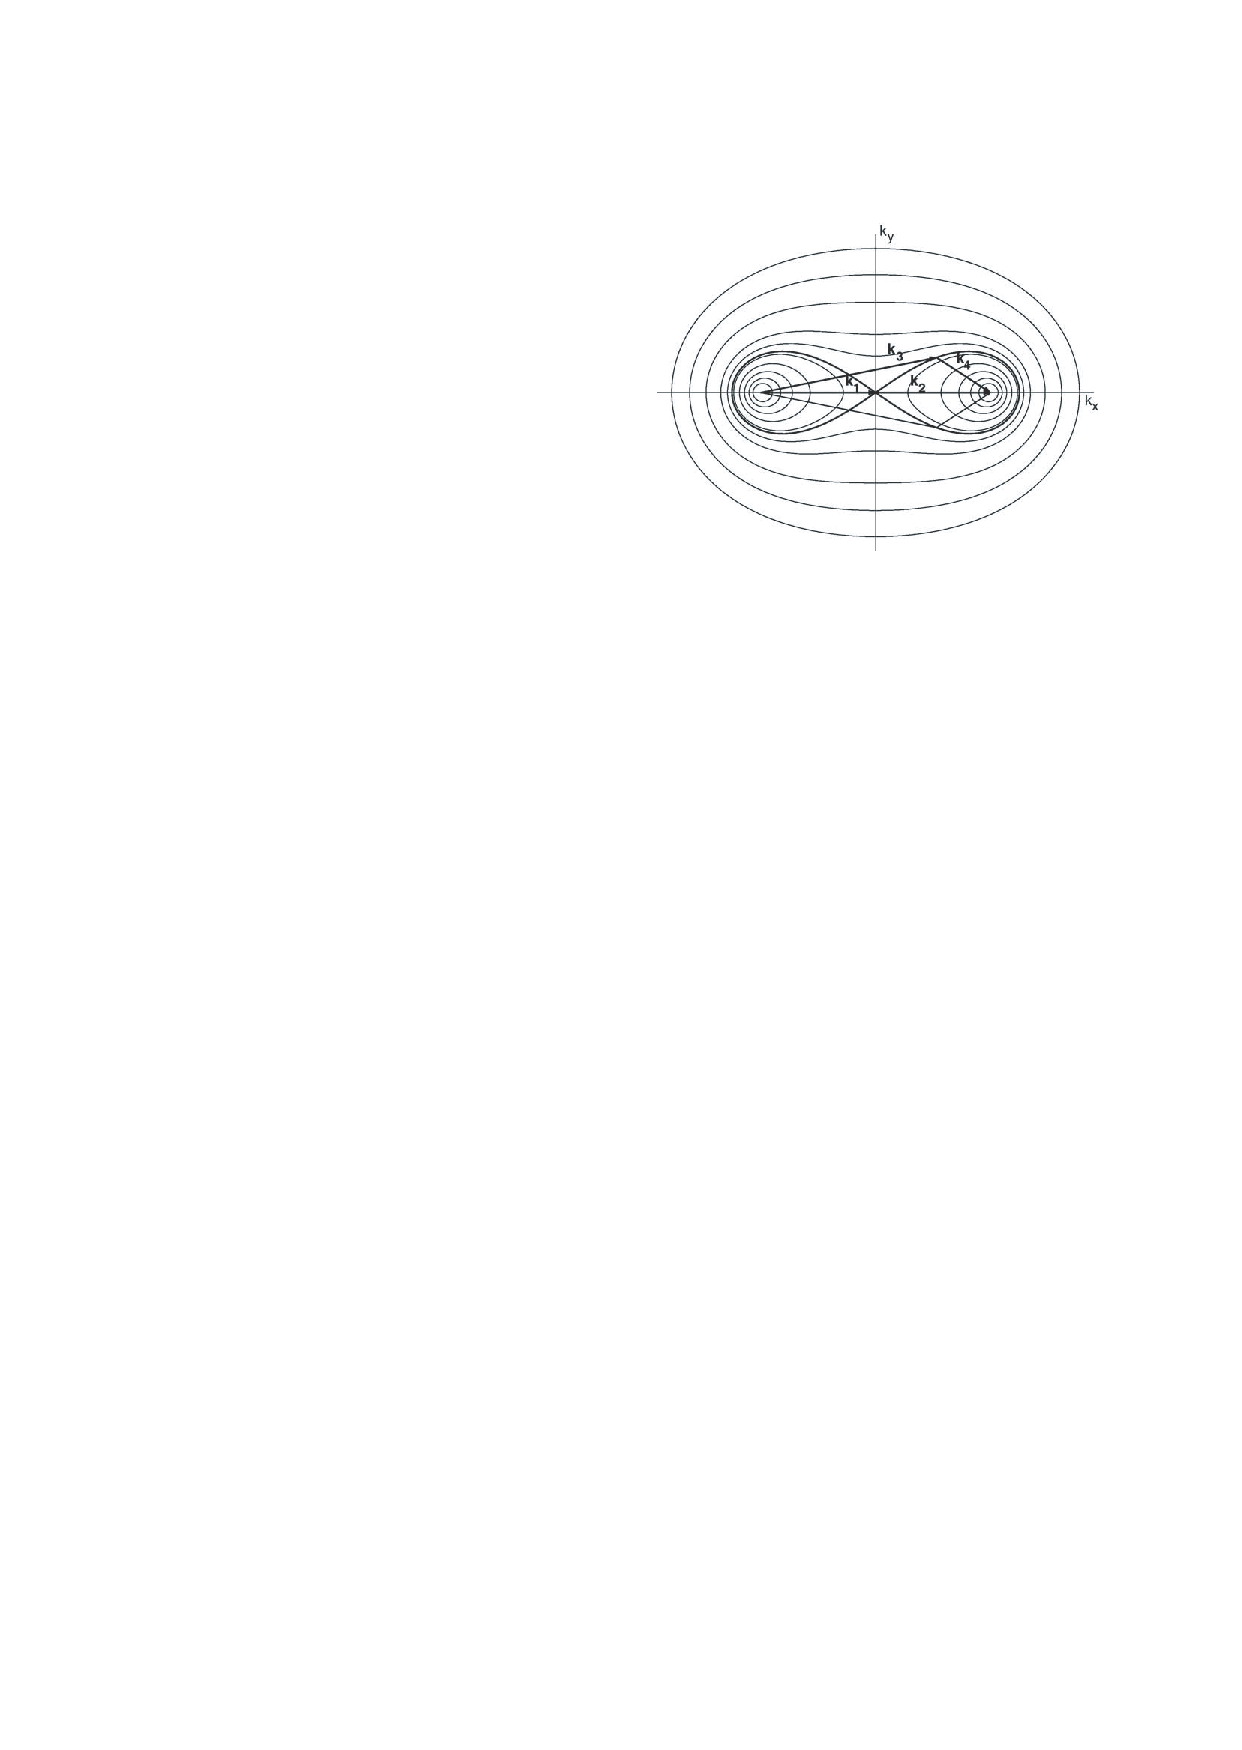
\includegraphics[width=0.68\textwidth]{FIGS_CH_SOURCETERMS/DIA_diagram.pdf}}
%\vspace{3.64in}
\caption{Geometric arrangement of wavenumbers that produce resonant interations in deep water, and particular 
case of the quadruplet used in the Discrete Interaction Approximation (DIA), taken from \cite{vanVledder2006}.}{
} \label{fig_DIA}
\end{figure}
%%%%%%%%%%%%%%%%%%%%%%%%%%%%%%%%%%%%%%%%%%%%%%%%%%%%%%%%%%%%% end of figure
A particular case corresponds to $\kb_1=\kb_2$, as in figure \ref{fig_DIA}. Any component $\kb_3$ that lies on the thick black curve shaphed like $\infty$, will interact resonantly 
with components $\kb_1$ and $\kb_4$. This was verified in the laboratory in the case where $\kb_3$ and $\kb_1$ are at right angles, 
with the creation of the new wave component $\kb_4$ \citep{McGoldrick&al.1966}. 


The fact that not all combinations of wavenumbers are resonant reduces 
the number of dimensions of the interaction space from 6 to 3.  In other words, the components with wavenumber vector $\kb_4$ interact with components 
$\kb_1$, $\kb_2$ and $\kb_4$ that follow some particular curves in spectral space. Assuming that the surface elevation is Gaussian makes it possible to neglect 
the correlations of 4 different wave trains \citep{Hasselmann1962},  giving a rate of change of the energy for time scales much larger that the wave period, 
\begin{eqnarray}
\frac{\partial E \left(\kb_4\right)}{\partial t}
    & = & S_{\mathrm{nl}} \left( \kb_4 \right) \nonumber\\
    & = & \int
    \left|T \left(\kb_1,\kb_2,\kb_3,\kb_4 \right)
    \right|^2
 \delta\left(\kb_1+\kb_2-\kb_3-\kb_4\right)
    \delta\left(\sigma_1+\sigma_2-\sigma_3-\sigma_4\right) \label{Snl:ch5}\\
 &&   \times \left\{E\left(\kb_1\right)E\left(\kb_2\right)
    \left[E\left(\kb_3\right)+E\left(\kb_4\right)\right]
    -E\left(\kb_3\right)E\left(\kb_4\right)
    \left[E\left(\kb_1\right)+E\left(\kb_2\right)\right]\right\}
%     {\mathrm d}\kb_1{\mathrm d}\kb_2{\mathrm d}\kb_3,
    \nonumber
\end{eqnarray}
where $\delta$ is always zero except $\delta(0)=1$, and the coefficient $T$ is an algebric expression similar to $A$ in eq. (\ref{eq:nl_A_simple}) but much more complex, and given by Herterich
et Hasselmann (1980\nocite{Herterich&Hasselmann1980}), or, with a simpler form, by  \cite{Zakharov1999}. 
The practical calculation of this coefficient and its integration requires a careful handling of singularities \citep[e.g.][]{Gorman2003}. 

The positive term $E\left(\kb_1\right)E\left(\kb_2\right)
    \left[E\left(\kb_3\right)+E\left(\kb_4\right)\right]$ in eq. (\ref{Snl:ch5}) comes from a third order amplitude squared, 
and the negative term $-E\left(\kb_3\right)E\left(\kb_4\right)
    \left[E\left(\kb_1\right)+E\left(\kb_2\right)\right]$ is due to the correlations between 
first and fifth order terms (see Part 3 for details). 
This negative part is critical to conserve the total wave energy. In general the coefficient $T$ decreases as the difference between wavenumbers 
is larger. In other words, the interaction of very different wavelengths or directions is much weaker than the interaction of
components that are very similar. A rough estimate of the time scale of spectral evolution is $\varepsilon^4
T_p$. 

Faster evolutions due to non-linear effects exist that are not represented by $S_{\mathrm{nl}}$. These faster changes are oscillations of the energies that 
do not contribute directly to the long term evolution of the wave spectrum. 

\subsection{Conservation properties}
The source term $S_{\mathrm{nl}}$ conserves the total wave energy, namely, 
\begin{equation}
E_{\mathrm{tot}}=\rho_w g \int E\left(\kb\right){\mathrm d}\kb
\end{equation}
as well as the wave momentum vector, which will be discussed further in the next chapter, 
\begin{equation}
\mathbf M^w=\rho_w g  \int
\kb \frac{E\left(\kb\right)}{\sigma} {\mathrm d}{\mathbf
k},
\end{equation}
and the wave action, 
\begin{equation}
A=\int  \rho_w g \frac{E\left(\kb\right)}{\sigma}
{\mathrm d}\kb.
\end{equation}
As we will see in chapter \ref{ch_current}, the conservation of wave action in general is related to the invariance of the phase-averaged physical situation by 
a change of the wave phases. In particular, wave action - and not wave energy - is conserved when waves propagate across current gradients without energy dissipation. 

The conservation of the two scalar quantities $A$ and $E$ in  a non-linear system imposes the presence of transfers of energy, also known as 'cascades', towards 
both short and long wave components \citep{Zakharov&Zaslavskii1982}. 
Indeed, once integrated over directions, $S_{\mathrm{nl}}(k)$ is the rate of change of the energy for a given wavelength. 
Assuming that there is only a transfer of energy from components with $k< k_t$ to shorter waves with $k > k_t$, we would have both 
\begin{equation}
\int_0^{k_t} S_{\mathrm{nl}}(k) \mathrm{d} k= - \int_{k_t}^{\infty} S_{\mathrm{nl}}(k) \mathrm{d} k
\end{equation}
 and 
\begin{equation}
\int_0^{k_t} S_{\mathrm{nl}}(k)/\sigma \mathrm{d} k= - \int_{k_t}^{\infty} S_{\mathrm{nl}}(k)/\sigma \mathrm{d} k,
\end{equation}
 which is not possible since the division by 
$\sigma$ makes the first integral relatively bigger than the second. 
Hence there is a flux of energy towards both long and short waves, which explains part of the increase in wavelength as the waves develop with time or fetch. 
Also, the conservation of momentum $\mathbf M^w$, further imposes that the energy transferred towards high frequency cannot be in the same direction, but rather in oblique 
or opposed directions. This property is tighly linked to the resonant conditions that is a consequence of the dispersion relation. 
Investigating the evolution of a narrow-peaked spectrum, \cite{Longuet-Higgins1976} showed that the energy tends to flow away from the peak towards high frequencies
at directions  $\arctan(1/\sqrt{2})$~rad~$\simeq 35^{\circ}$ (figure \ref{fig_Snl_dir}). Under the effect of nonlinear interactions alone, a narrow 
spectrum thus tends to have a split tail with two peaks separated by about  70$^{\circ}$, which agrees with the observations 
of wind sea spectra at frequencies $1.5 f_p < f < 2 f_p$ \citep{Hwang&al.2000b,Long&Resio2007}, as shown in figure \ref{bimodal}.
%%%%%%%%%%%%%%%%%%%%%%%%%%%%%%%%%%%%%%%%%%%%%%%%%%%%%%%%%%%%%%%%% figure
\begin{figure}
\centerline{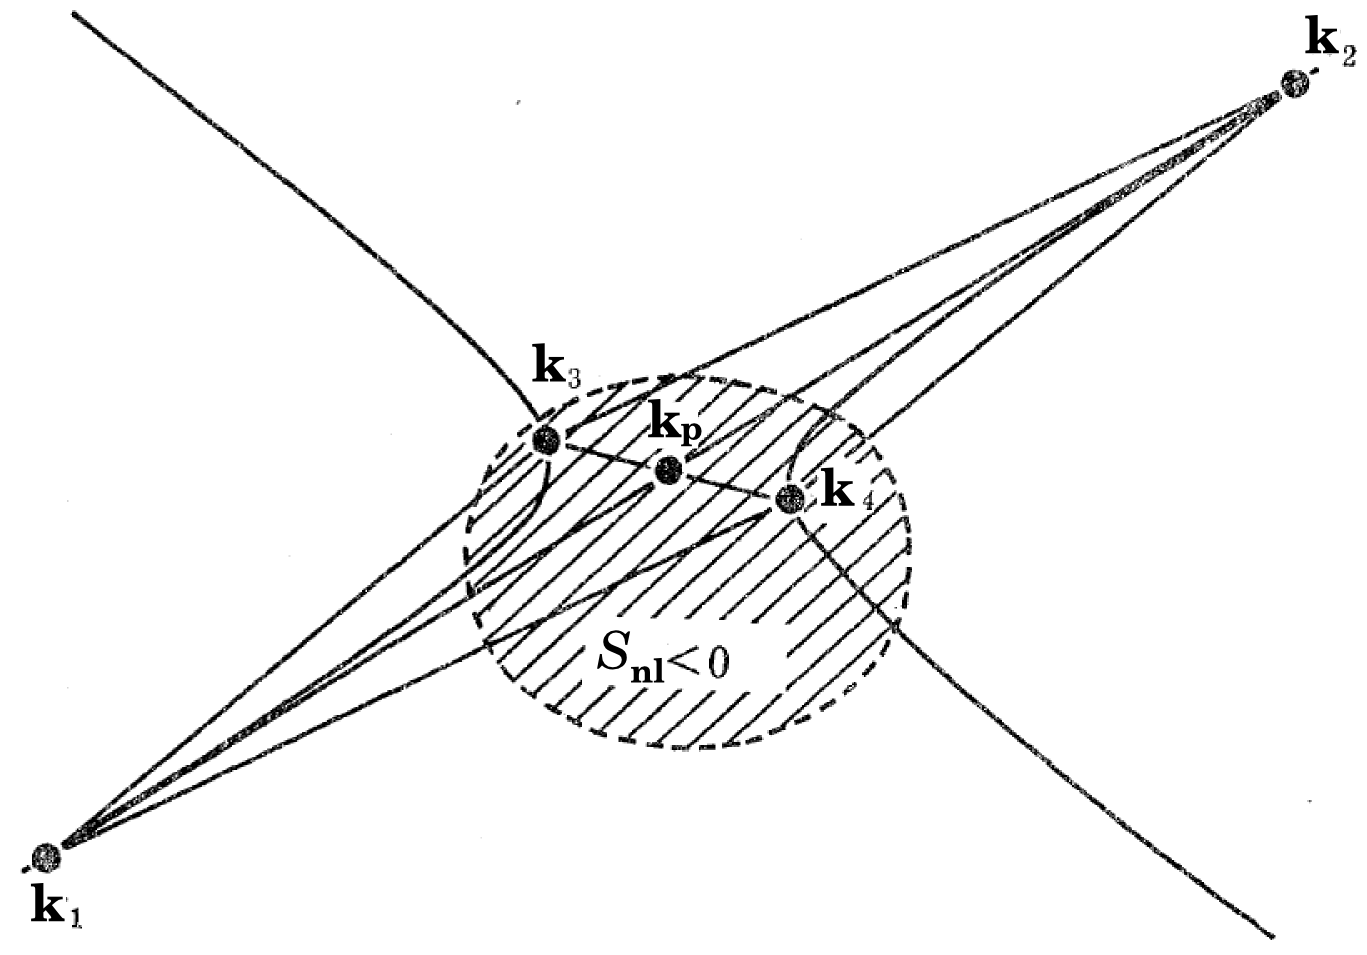
\includegraphics[width=0.50\textwidth]{FIGS_CH_SOURCETERMS/Snl_directions_v2.png}}
%\vspace{3.64in}
\caption{Non-linear interactions and bimodal spectral distributions.}{The interaction of wave components with wavenumber vectors 
$\kb_1$, $\kb_2$, $\kb_3$ and $\kb_4$, when $\kb_3 \simeq \kb_4$. Since $\kb_1+\kb_2=\kb_3+\kb_4$, the 4 wave vectors make a parallelogram. 
taking $\kb_3$ and $\kb_4$ symmetric about the spectral peak $\kb_p$ and taking the $x$-axis in the direction of   
 $\kb_p$, one gets $k_{p,y}=0$ and $k_1 = \sqrt{k_p^2+ 2 k_p \Delta k_{1,x}+ \Delta k_{1,x}^2+\Delta k_{1,y}^2}$, the latter equation also 
applies to the three other wave vectors. Expanding for small values of 
$X_1=\Delta k_{1,x}/k_p$ and $Y_1=\Delta k_{1,y}/k_p$ gives $\sigma_1 =\sqrt{g k_1} \simeq \sqrt{g k_p} \left( 1 +0.5 X_1 - 0.125 X_1^2 + 0.25 Y_1^2 \right)$,.
The resonant conditions read $X_1+X_2=0$ $Y_1+Y_2=0$ and, for the frequencies $\sigma_1+\sigma_2=2 \sigma_p (1+\alpha)$ becomes 
$2 Y_1^2 - X_1^2 = 8 \alpha$. That is the equation of an hyperbola with asympotes at angles 
$ \pm \arctan(1/\sqrt{2})$ relative to the $x$-axis \citep[figure adapted from][]{Longuet-Higgins1976}
.} \label{fig_Snl_dir}
\end{figure}
%%%%%%%%%%%%%%%%%%%%%%%%%%%%%%%%%%%%%%%%%%%%%%%%%%%%%%%%%%%%% end of figure


Without forcing from the wind and assuming that the dissipation occurs only at the smallest scales, the wave spectrum tends to evolve 
towards a self-similar shape known as the Kolmogorov-Zakarov spectrum, with a decay towards high frequencies that is proportional to $f^{-4}$. 
In reality, the presence of forcing and dissipation at the dominant scales makes the wave spectra different from this self-similar solutions. 

\subsection{Other properties of wave-wave interactions}
Besides the fluxes towards both ends of the spectral domain, the non-linear interactions
also have a very strong local smoothing effect. If one takes a spectrum near equilibrium and introduces a 
local perturbation, the 4-wave interactions will very rapidly remove this disturbance
giving a smooth spectrum. This smoothing is faster for steeper waves. For a wind sea, this can happen in less than 100 periods,  (figure \ref{fig_YoungVledder}), which is 
much faster than the theoretical dimensional argument saying that $S_{\mathrm{nl}}$ acts on a time scale of $\varepsilon^6 T_p$. In the case of swells, 
with a much weaker steepness, it is possible that the interactions produce a significant broadening of the directional spectrum, without a noticeable shift in 
frequency  (T.H.C. Herbers, personal communication, 2001). 
%%%%%%%%%%%%%%%%%%%%%%%%%%%%%%%%%%%%%%%%%%%%%%%%%%%%%%%%%%%%%%%%% figure
\begin{figure}[htb]
\centerline{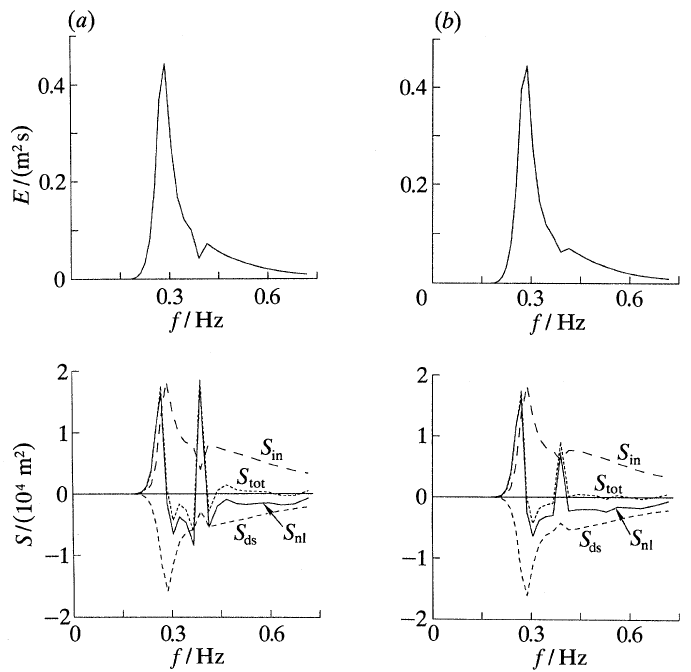
\includegraphics[width=0.70\textwidth]{FIGS_CH_SOURCETERMS/Young_Vledder_1993.png}}
%\vspace{3.64in}
\caption{Illustration of the smoothing effect of non-linear interactions.}{A spectrum with a gap, evolves rapidly 
towards a smooth spectrum. Top-left: initial spectrum, right: spectrum after 3 minutes, which is less than 100 dominant periods. Bottom: 
source terms for wind generation $S_{\mathrm{in}}$, wave-wave interactions $S_{\mathrm{nl}}$, and dissipation $S_{\mathrm{ds}}$. Figure taken from \cite{Young&VanVledder1993}
.} \label{fig_YoungVledder}
\end{figure}
%%%%%%%%%%%%%%%%%%%%%%%%%%%%%%%%%%%%%%%%%%%%%%%%%%%%%%%%%%%%% end of figure

\subsection{Practical calculation of wave-wave interactions}
The calculation of the full integral $S_{\mathrm{nl}}$ is unfortunately a little too expensive today for operational wave forecasting, 
except for large scale coarse models, due to the three-dimensional integral needed for each spectral component and at each grid point where the 
source terms are evaluated. Such calculations are thus confined to research applications. Operational wave models use some form of approximation, and the Discrete 
Interaction Approximation by \cite{Hasselmann&al.1985} is the most common. That approximation preserves the conservation properties of the full integral 
by using only a subset of the resonant quadruplets  $\kb_1$,  $\kb_2$, ${\mathbf
k}_3$, et $\kb_4$. 
The resonance conditions $\kb_4=\kb_1+\kb_2-\kb_3$ and $\sigma\left(k_4\right)=\sigma_1+\sigma_2-\sigma_3$ 
mean that for a given $\kb_1+\kb_2$, $\kb_3$ must be on the curve where $\kb_1$ lies: each curve corresponds to a fixed value of $\sigma_1 + \sigma_2$.
The DIA parameterization uses a single configuration  ${\mathbf
k}_1=\kb_2=\kb$, $k_3 = (1+\lambda)^2 k$ and
$\sigma_1+\sigma_2=\gamma \sigma$, which imposes $k_4 =
(1-\lambda)^2 k$. This DIA, as adjusted by \cite{Hasselmann&al.1985b}, uses  $\lambda=0.25$ et $\gamma
= \sqrt{2}$. 
The angle of the $\infty$-shaped curve near the origin with the $x$-axis, when $\kb_3 \simeq \kb_1$ is the same 35$^{\circ}$ angle as in figure \ref{fig_Snl_dir}. Each 
curve corresponds to a different value of $\gamma$.
The original form of the DIA is only valid in deep water. 

The shape of  $S_{\mathrm{nl}}$ produced by the DIA can differ significantly from the exact solution. It has been adjusted to give the right order 
of magnitude for the transfer of energy to low frequencies in a wind sea, which is very important for the wave development. That choice, has some side-effects on other unconstrained
parameters such as the directional wave distribution which is too broad for  $1.5 <f_p <f<4 f_p$.

Several intermediate methods have been developed with some already used in operational wave forecasting \citep[e.g.][]{Komatsu&Masuda1996}. 


\section{Dissipation\label{section_whitecap}}
Many processes contribute to the dissipation of wave energy, or more exactly, the conversion of 
mechanical wave energy into other forms of energy, in particular turbulence in the water and air. 

Wave breaking is generally the most important sink of energy for wind seas. In the case of periodic waves, breaking results from 
an instability that develops near the wave crest when the orbital velocity appraoches the phase speed\footnote{In the case of a stationnary 
wave, instability occurs when the vertical acceleration approaches $g$.}. This criterion gives a maximum possible wave steepness that 
is 
\begin{equation}
H_{\max}/L \simeq 0.14 \label{eq:Miche_limit}
\tanh(kD)    
   \end{equation}
as first determined by \cite{Miche1944d}. 
 The factor $\tanh(kD)$ happens to be also the ratio between the amplitude of elevations $a$ and the amplitude of the orbital velocities at the 
surface in the case of linear waves. It is likely that a similar criterion applies to random waves. Indeed, water moving forward faster than the crest will 
shortly find itself over air and ready to overturn. In deep water, the Miche criterion (\ref{eq:Miche_limit}), gives the Stokes limit, $k a_{\max} = \pi H_{\max}/L = 0.44$. 

Laboratory observations by 
\cite{Melville&Rapp1988} and \cite{Stansell&MacFarlane2002} show that non-stationary breaking waves have 
orbital velocities $u$ that approach the phase speed. One of the important difficulties is to relate this orbital velocity to the wave spectrum, because, 
for real and thus nonlinear waves, 
$u$ increase much faster than $a$ when approaching the breaking limit. 
Also, breaking is defined for individual waves, which are not easily related to the spectrum. Many authors have sought criteria for wave breaking 
based on the vertical acceleration, but this is not a good indicator of breaking  (e.g.
Holthuijsen and Herbers 1986\nocite{Holthuijsen&Herbers1986}).
%%%%%%%%%%%%%%%%%%%%%%%%%%%%%%%%%%%%%%%%%%%%%%%%%%%%%%%%%%%%%%%%% figure
\begin{figure}[htb]
\centerline{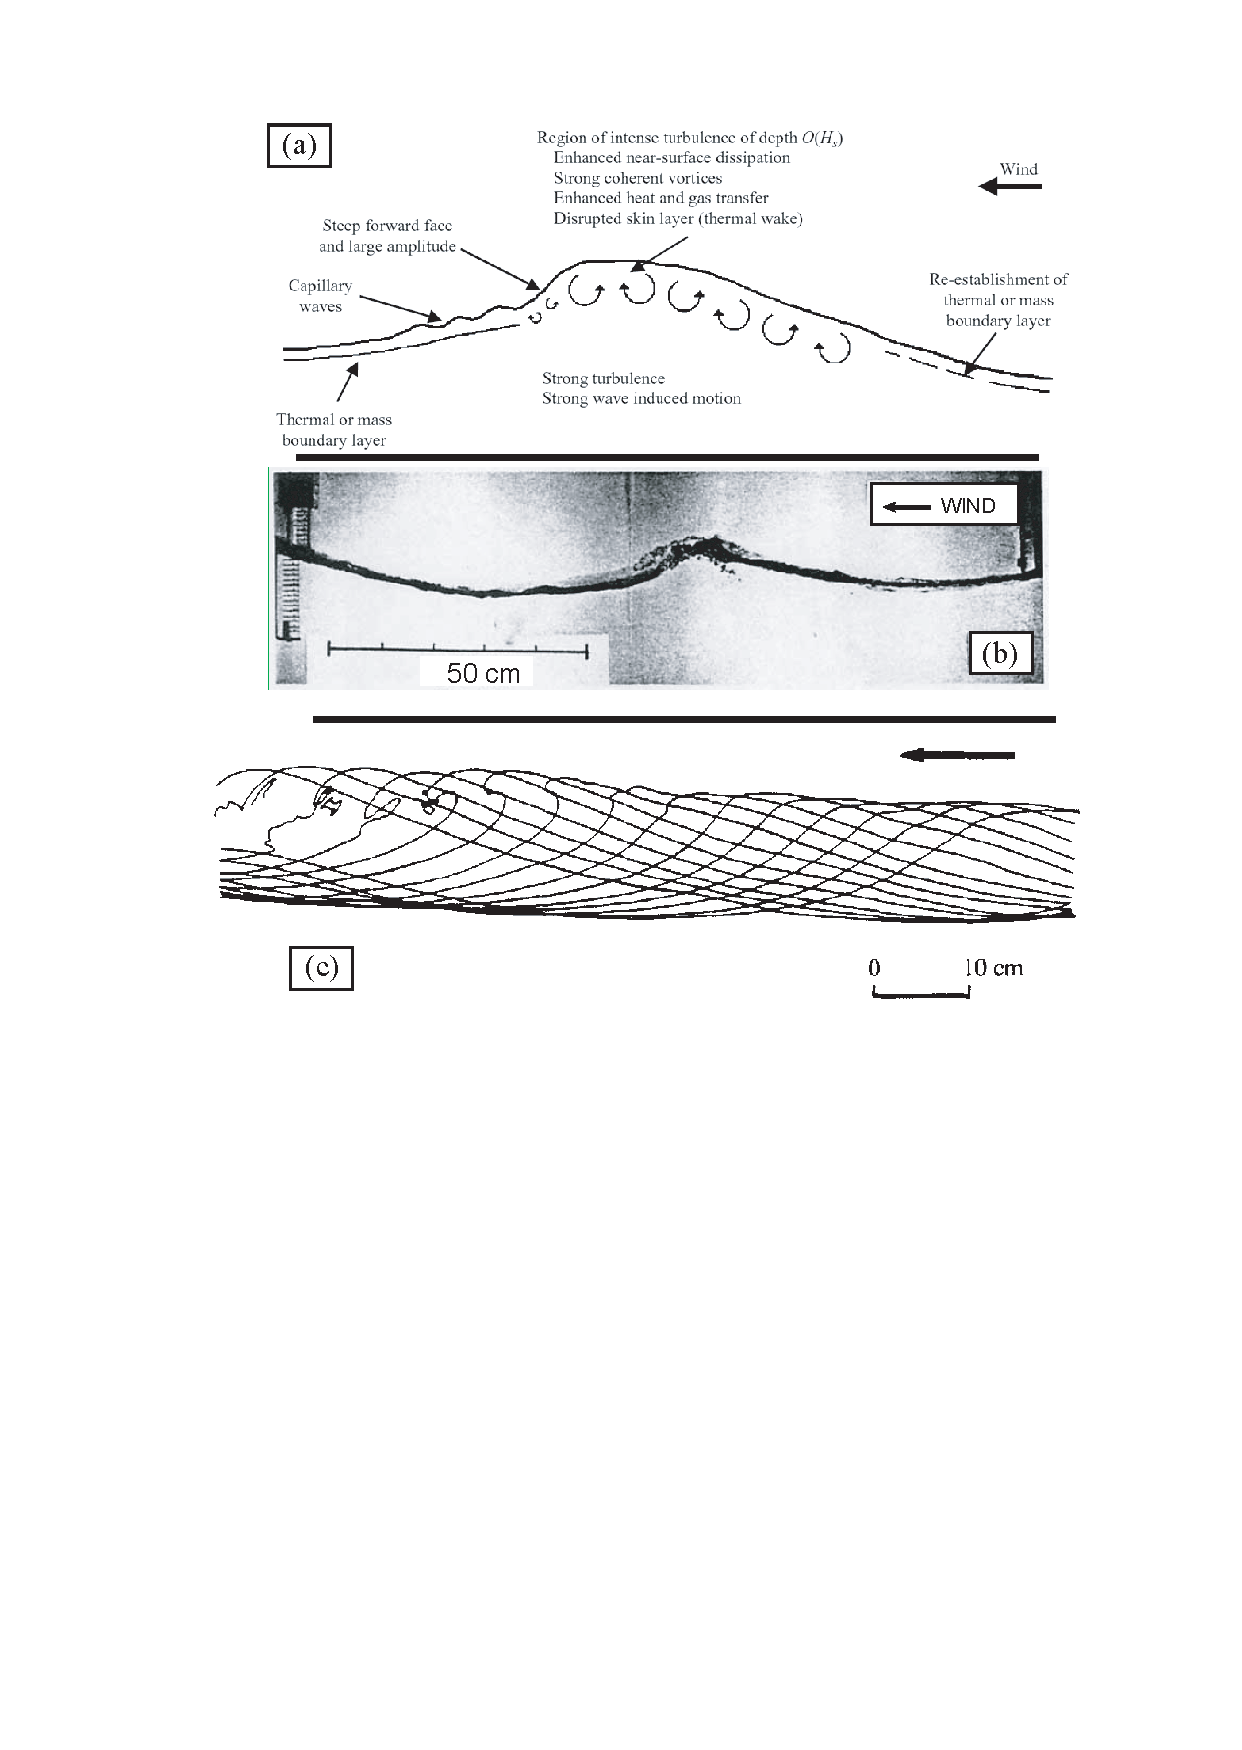
\includegraphics[width=0.6\textwidth]{FIGS_CH_SOURCETERMS/breaking_basic.pdf}}
%\vspace{3.64in}
\caption{Features of breaking waves from short to longer waves.}{(a) Schematic of a micro-breaking waves viewed sideways, the vertical scale 
of the boundary layer is exaggerated \citep[from][\copyright Cambridge University
Press]{Siddiqui&Loewen2007}, (b) breaking of a short wave with entrainment of air at the crest \citep[from][]{Koga1982}, (c) evolution 
of a breaking wave in the case of a plunging breaker with one wave profile every  0.04~s
\citep[from][\copyright Cambridge University
Press]{Bonmarin1989}
}.\label{figbreaking1}
\end{figure}
%%%%%%%%%%%%%%%%%%%%%%%%%%%%%%%%%%%%%%%%%%%%%%%%%%%%%%%%%%%%% end of figure


\subsection{A classification of breaking waves}
Breaking waves of different sizes look different. The shortest gravity waves, with wavelengths $0.1 <
L < 1$~m (i.e.  $f > 1.25$~Hz) do not make any bubbles. This is because an increase in the area of the  air-water
interface requires an energy that is the surface tension $T$ times the excess surface, hence the short waves do not have enough energy to make bubbles 
when the break. Instead, short waves produce micro-breakers \citep{Banner&Phillips1974}
that are characterized by a strong curvature of the surface and the generation of capillary ripples on the forward face ahead of the breaking point.  
These capillary waves are strongly damped by viscosity that absorbs a large part of the energy lost during breaking. 
Observations reveal that short waves break very often, with a probability that increases from  11\% for a wind speed of 4{\d}5 m/s to 80\% for 7{\d}4m~s$^{-1}$
\citep{Siddiqui&Loewen2007}.
These micro-breakers play an important role in setting the surface temperature and the gas fluxes at the air-sea interface because they disrupt the viscous surface layer (figure \ref{figbreaking1}.a).

Longer waves are energetic enough to produce bubbles with a particular noise. This ambiant noise is an important factor 
in the performance of sonar systems \citep[e.g.][]{Lu&al.1990,Ma&al.2005}. Injecting the bubbles at depths also requires a conversion of kinetic 
energy into potential energy, that can take up as much as half of the energy lost in the whole breaking process \citep{Lamarre&Melville1991}. It should be noted
that long waves can contribute to the breaking of short waves, either because the long waves are breaking or because they produce a 
straining of the short waves that locally increases the short wave steepness.
Wave breaking of all scales produce vorticity in the water column which is important for upper ocean mixing, in particular for the diurnal cycle of sea surface 
temperature. 

Several types of breakers are usually defined. When the breaking wave is quasi-stationary 
with a gentle forward slope, it is a spilling breaker. A steeper waves that trap a tube of water near the crest, is a plunging breaker (figure
\ref{figbreaking1}.c). Finally a waves that rapidly collapses on a steep shoreline is surging breaker. 



\subsection{Parameterizations of dissipation due to breaking in shallow water}
\subsubsection{Dissipation of the total wave energy\label{sds:energy}}
Near the shore or on offshore shoals, the water is shallow enough that the dominant waves are not dispersive. In that 
case the question of wave breaking is greatly simplified by considering the total energy $E_t$ instead of the spectrum. 
Since waves near the shore often have a well-defined direction we may consider that the wave energy is radiated in a single direction, 
that of the spectral peak. 
By analogy with a hydraulic jump, as detailed in Part 3,
the rate of energy dissipation per unit surface is 
\begin{equation}
    \epsilon(H,D,T) \simeq \frac{1}{L}\epsilon_1(D-H/2,D+H/2) \approx \frac{1}{4}  \rho g \frac{\left(B H \right)^3}{D T}
\label{epsi_shallow_mean}
\end{equation}
where $B$ is a tuning factor that is close to 1... empirical adjustments are often useful to produce accurate simulations, and this is one of the better constrained 
coefficients. Obviously, as $B$ comes to the third power, a small change in $B$ can be a significant change in the modeled dissipation rate. 




\subsubsection{Effect of wave height distributions}
Since the wave height $H$ is very important for the dissipation rate, we should 
determine what is the period and height of the waves that actually break. Experimental data shows that the breaking waves have a probability distribution 
$p_B(H,T)$ that is different from the distribution $p(H,T)$ of all -- breaking or not -- waves. We can define 
a weighting function $W$ that gives the breaking wave distribution from the full wave distribution,
\begin{equation}
 p_B(H,T)=p(H,T)W(H,T).
\end{equation}

The dissipation rate per unit time and per unit horizontal surface is thus an average over all heights and should equal the sum of all spectral 
components,
\begin{equation}
  \epsilon_{\mathrm{tot}}=
  \int \epsilon(H,D,T) W(H,T) p\left(H,T\right) \mathrm{d} H=\rho g  \int_\kb S_{\mathrm{dis}}\left(\kb\right) \mathrm{d} \kb .\label{Sds_tot_BJ}
\end{equation}


In deep water, neither the orbital velocity nor the pressure gradient are uniform over the vertical. 
The energy flux is thus clearly different from the shallow water value. 
Hence the depth $D$ that appears in the dissipation rate $\epsilon$ should be -- at the very least -- replaced by a relevant length scale $\widetilde{h}$. 
\cite{Chawla&Kirby2002} proposed to use $\widetilde{h}=\tanh(kD)/k$  which goes to $D$ when $kD$  goes to zero. In order to reproduce the wave evolution 
in both deep and shallow water, \cite{Filipot&al.2010b} have redefined  $B$ as a function of $kD$ with $B=0.185 / \tanh[(kD)^{1.5}]$. 
This leads to 
\begin{equation}
    \epsilon(H,D,T) = \frac{1}{8 \pi} \rho g k \left(B H \right)^3 \sqrt{\frac{gk}{\tanh(kD)}} \label{eps_CK2002}
\end{equation}
The choice of  $\widetilde{h}$  can be debated and should be determined from an energy balance such as  eq. (\ref{epsi_shallow_mean}). 

%%%%%%%%%%%%%%%%%%%%%%%%%%%


\subsubsection{Breaking wave statistics in shallow water\label{TG1983}}
Finally, the dissipation rate requires a definition of  $W(H,T)$ and $p\left(H,T\right)$. 
In shallow water, the energy is usually integrated across frequencies, and  in that case we only need $W(H)$ and $p\left(H\right)$. The latter is often taken to be the Rayleigh distribution $p_R$ (figure \ref{fig:Rayleigh}). 
For $W$, two different choices have been made. The first choice by \cite{Battjes&Janssen1978} 
is based on the idea that all breaking waves have the same height corresponding to the depth limitation  
$H=\gamma  D$ in which $\gamma$ is a known constant, and the probability of occurence of these waves is simply given by the Rayleigh distribution, namely 
$Q_B=p_R(h > \gamma D)$. The resulting functions $p(H)$ and $W(H)$ thus have a singularity at $H= \gamma D$. On the problem of this first approach is 
that it can lead to unphysical parameters such as $Q_B > 1$, which is not very nice for a probability 
\citep{Janssen&Battjes2006}. 

The second choice is an empirical determination of  $W$  from observations. After days of counting waves passing by a fixed location in the surf zone, 
\cite{Thornton&Guza1983} have proposed the empirical expression
\begin{equation}
    W(H)=\left(\frac{H_{\mathrm{rms}}}{\gamma D}\right)^4
\end{equation}
where $\gamma$ plays a role similar to the $\gamma$ in  \cite{Battjes&Janssen1978}. One reason why they chose this particular form, is that it allows an analytic 
integration of eq. (\ref{Sds_tot_BJ}) that gives,
\begin{equation}
    \epsilon_{\mathrm{tot}} = \frac{3}{16} \pi^{1/2} \rho g \frac{B^3}{\gamma^4 D^5}f_p
    H_{\mathrm{rms}}^7.
\end{equation}
in which $f_p$ is the peak frequency. 

\subsection{Breaking wave statistics and dissipation rates in deep water}
Many applications, including underwater acoustics, remote sensing and the investigation of 
air-sea fluxes, rely on some characterization of breaking waves. The investigation of breaking waves 
has been limited for a long time ot the estimation of the whitecap coverage in which the active part and the residual 
foam was separated  \citep[e.g.][]{Monahan&Woolf1989}. This coverage was found to be strongly related to the wind speed, 
with an increase from very low values for pour $U_{10} < 7$~m~s$^{-1}$, to about 1~\% for $U_{10} \simeq
10$~m~s$^{-1}$,  6~\% for $U_{10} \simeq 20$~m~s$^{-1}$, and much more for yet higher wind speeds. In fact, 
these variations in foam coverage and aspect are the basis of the Beaufort scale (see table \ref{table_beaufort}) that 
is still used to determine the wind speed from a visual inspection of the sea. 

Wave breaking can also occur without any wind, due to the convergence of wave energy associated to 
current gradients or the bottom topography.  Most authors have distinguished a 'depth-induced'
wave breaking that occurs near the shore in the 'surf zone', from the 'whitecapping' that occurs in deep water, usually 
in the presence of wind. This distinction can be fuzzy in the case of shallow tidal flats, which is why we preferred 
to have a single breaking definition \citep{Filipot&Ardhuin2012}. 

The fraction of sea surface 
covered by foam or the breaking probability used in shallow water is not sufficient to fully characterize wave breaking. 
Hence \cite{Phillips1985} proposed a spectral 
description of breaking and introduced the breaking spectrum 
$\Lambda$, which is the density of breaking crest length per unit surface and per unit vector speed $\cb$ of the breaking fronts. 
%%%%%%%%%%%%%%%%%%%%%%%%%%%%%%%%%%%%%%%%%%%%%%%%%%%%%%%%%%%%%%%%% figure
\begin{figure}[htb]
\centerline{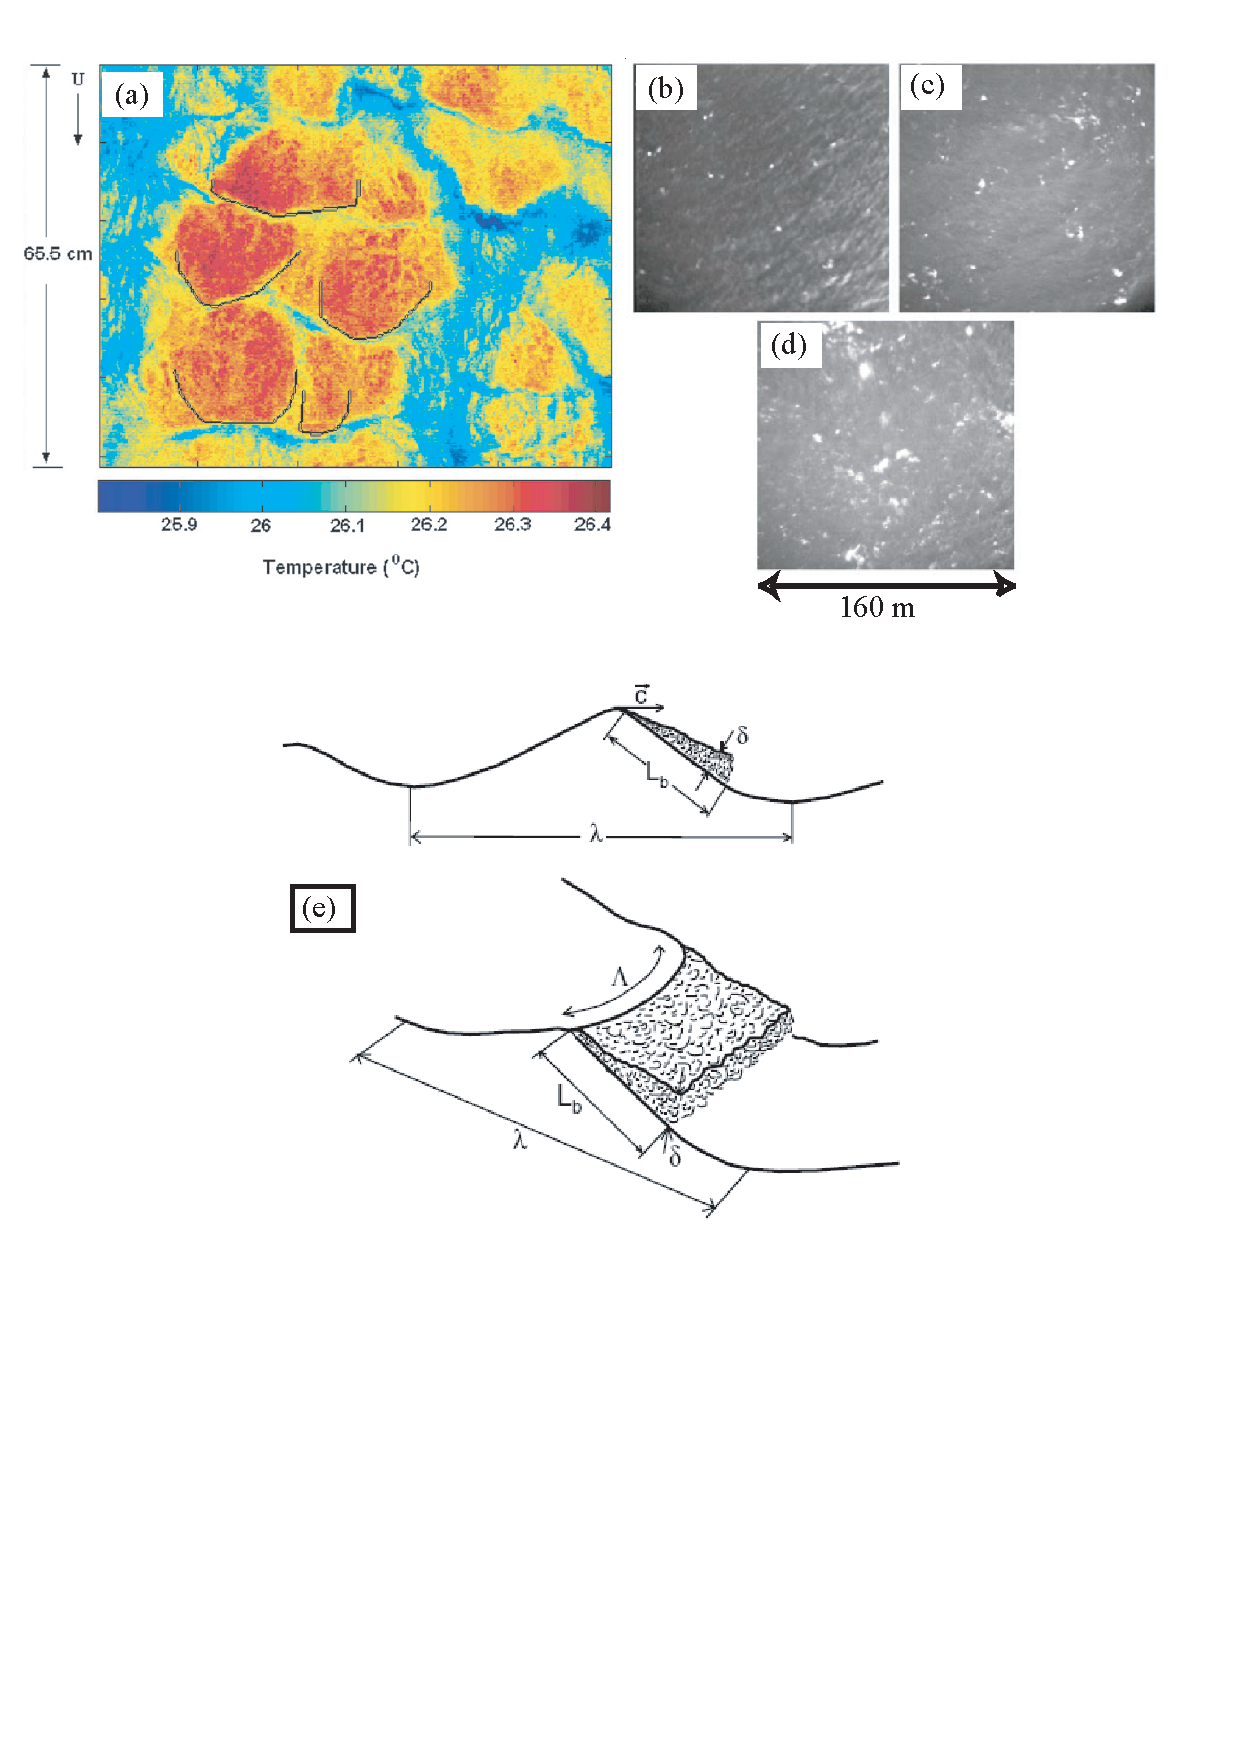
\includegraphics[width=0.8\textwidth]{FIGS_CH_SOURCETERMS/breaking_lambda.pdf}}
%\vspace{3.64in}
\caption{Breaking fronts}{(a) Detection of breaking front, in black, using infrared imagery of micro-breakers  (picture from 
Jessup and Phadnis 2005\nocite{Jessup&Phadnis2005}) , (b), (c), (d) foam coverage for wind speeds of 7, 10 and 14~m~s$^{-1}$
(Melville and Matusov 2002\nocite{Melville&Matusov2002}), and (e)
schematic defining $\Lambda$ (from Reul and  Chapron 2003\nocite{Reul&Chapron2003}).}\label{figlambda}
\end{figure}
%%%%%%%%%%%%%%%%%%%%%%%%%%%%%%%%%%%%%%%%%%%%%%%%%%%%%%%%%%%%% end of figure
With this definition, the length  $\Lambda (\cb) {\mathrm d}c_x {\mathrm d}c_y$
is the total length of all breaking fronts per unit sea surface that move at a speed  $\cb=(c_x,c_y)$ within a speed interval 
${\mathrm d}c_x$ and ${\mathrm
d}c_y$. In general $c$ is about 0.8 times the phase speed $C$ of the dominant waves that are breaking, 
due to modulation effects \citep{Banner&al.2014}. Such a decomposion of the breaking 
waves was motivated by the observation by \cite{Duncan1981,Duncan1983} in the laboratory 
that the dissipation is proportional to $c^5$. 

Other interesting quantities derived from $\Lambda$ include the fraction of the sea surface 
wiped by breaking fronts per unit time $\int c \Lambda {\mathrm d}c_x {\mathrm
d}c_y$. Assuming that the breaking waves have self-similar shapes, $\Lambda$ can also be used to 
provide a an estimate of the mean foam thickness \citep{Reul&Chapron2003}.

The investigation of breaking wave properties has thus focused onthe 
estimation of $\Lambda$ from observations or models. This is not an easy task, requiring 
high resolution video data in both optical and infrared as illustrated in figure \ref{figlambda} \citep[e.g.][]{Sutherland&Melville2013}.
More classical measurements of surface elevation time series have also been associated to a visual or acoustic 
indentification of breaking waves \citep{Banner&al.2000,Babanin&al.2001,Manasseh&al.2006}. These studies 
have led to the conclusion that the breaking of dominant waves is not associated to a fixed threshold, but that statistically,
the probability of breaking waves can be predicted from the energy level of dominant waves. 
There is a fixed threshold, when the energy is put in non-dimensional form, over which breaking occurs. 
There is thus a link between the breaking probability and the 'saturation' spectrum $B(\kb)$ introduced by \cite{Phillips1985} and 
defined by
\begin{equation}
B\left(k,\theta\right)=\int_{\theta - \Delta \theta}^{{\theta +
\Delta \theta}} \int_{k-\Delta k}^{k+\Delta k}
\cos^p(\theta-\theta') k^2 E(k,\theta') \mathrm d k \mathrm d
\theta' \label{defBofk}.
\end{equation}
%%%%%%%%%%%%%%%%%%%%%%%%%%%%%%%%%%%%%%%%%%%%%%%%%%%%%%%%%%%%%%%%% figure
\begin{figure}
\centerline{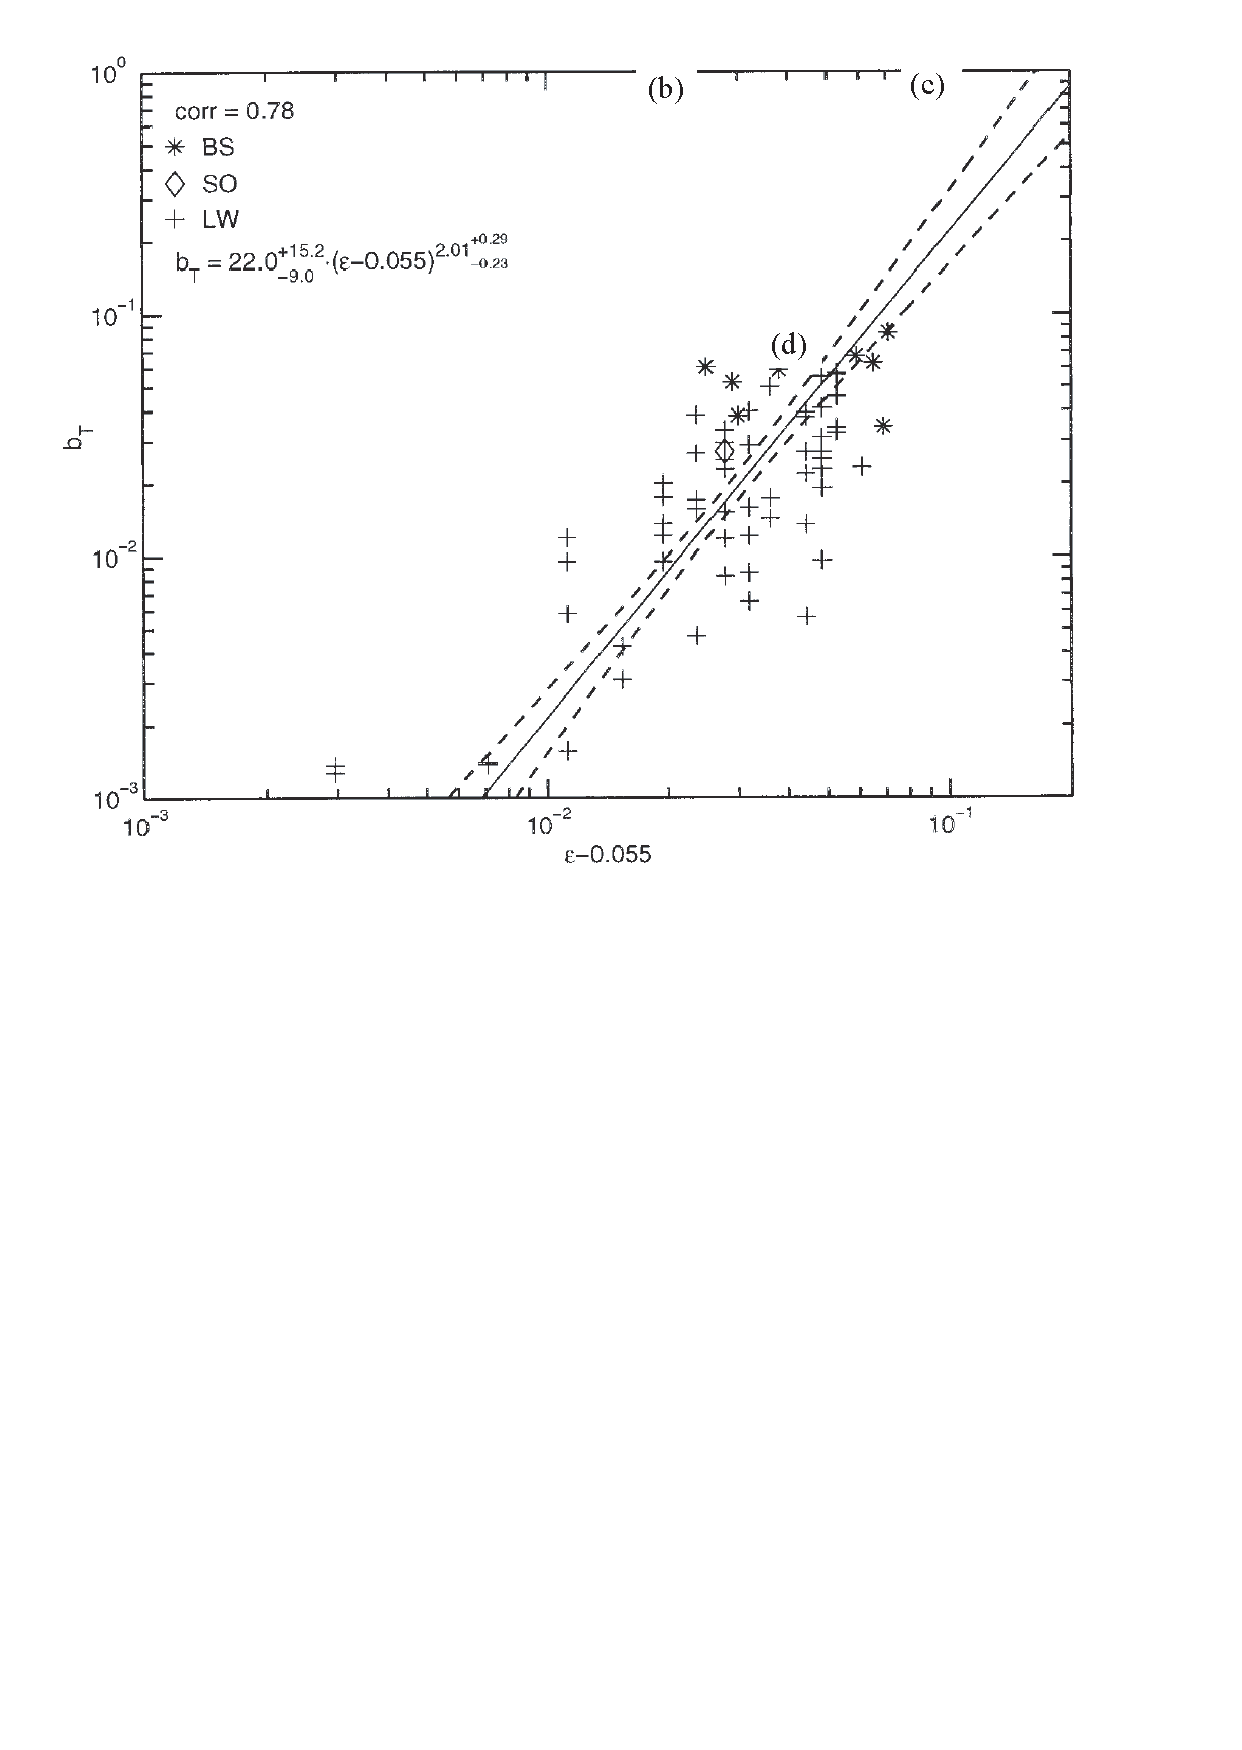
\includegraphics[width=0.7\textwidth]{FIGS_CH_SOURCETERMS/breaking_threshold.pdf}}
%\vspace{3.64in}
\caption{Breaking probability and saturation}{The probability of breaking of dominant waves $b_T$ is linked to the 
steepness of the dominant waves $\varepsilon$ which is related 
to the saturation $\varepsilon^2\simeq 4 B\left(\kb\right)$ with $\Delta
\theta =\pi$ and $\Delta k \simeq 0.6 k$. The threshold over which breaking is observed is $\varepsilon=0.055$, 
which corresponds to $B\left(\kb\right) \simeq 1\times
10^{-3}$.}\label{figsaturation}
\end{figure}
%%%%%%%%%%%%%%%%%%%%%%%%%%%%%%%%%%%%%%%%%%%%%%%%%%%%%%%%%%%%% end of figure

As pointed out by Phillips
(1984\nocite{Phillips1984}), using a local definition of $B$ with $\Delta \theta$ and $
\Delta k$ very small makes sense only if the spectrum is relatively smooth. Indeed, for a narrow spectrum,   $B$
could be very large with very small amplitude waves, even going to infinity for 
monochromatic waves.  In their analysis \cite{Banner&al.2000} used $\Delta \theta
=\pi$, $p=0$ and $\Delta k \simeq 0.6 k$. In fact, it is difficult to investigate breaking statistics for small values of 
$\Delta \theta$, due to the greater statistical uncertainty. In practice the breaking probability is 
associated to the presence of steep waves, and these can exist only if wave trains with neighboring wavenumbers and directions 
can interact to form wave groups that live long enough to let the waves evolve towards breaking. The basic interaction is first 
a linear superposition, and the eventual evolution up to breaking is obviously nonlinear \citep[e.g.][]{Song&Banner2002}. 

Besides, the fact that 
$B$ has no dimensions suggests that breaking mainly depends on the shape of the waves, while other factors (wind, current ...) are 
only secondary.   After a first demonstration for dominant waves, a threshold for $B$ has also been proposed for the shorter 
compoents \citep{Banner&al.2002}.

We note that if $B$ is constant then the wavenumber spectrum integrated over directions decays like $k^{-3}$ and, 
assuming that waves are linear, the frequency spectrum decays like $f^{-5}$. Besides, a constant non-dimensional spectrum 
means that all the scales have the same shape: the waves are self-similar. We had found before that non-linear wave-wave 
interactions tend to impose a $f^{-4}$ shape to the spectrum. Well, this shape is not possible beyond some frequency 
where it crosses the $f^{-5}$ asymptote as the steepness of the waves must be limited by breaking. 



\subsection{A spectral approach} 
In order to decompose the overall dissipation rate $ \epsilon_{\mathrm{tot}} $ across the 
spectrum one can use an empirical approach by distributing the total dissipation with 
particular shape factor, e.g. using a distribution of the dissipation proportional to  $f^2$, as is often done 
for depth-induced breaking in the surf zone. In that case, waves are almost not dispersive and it makes sense to 
combine all components. 

In other conditions, it makes sense to decouple the disspation of wave components that 
have very different wavelengths and directions. In that case we can define a parametrization 
that is consistent with the data of \cite{Banner&al.2000}. 

A first step is thus to determine the breaking probability for different wave 'scales': these scales are spectral regions
within which the frequencies and directions are close enough that their superposition 
produce well defined wave groups with long-lived wave crests that have enough time evolve towards breaking. 
We can then link the breaking probability to  $B$ which, taking $p=2$ is a non-dimensional variance of the orbital velocity. 

The second step is to atribute to each spectral component that contribute to a given scale 
the breaking probability and dissipation rate. This gives a dissipation source term 
\begin{equation}
  S_{\mathrm{dis,s}}\left(\kb\right)=
 \int_\kb h(\kpb-\kb) P \left(B(\kpb)\right)q\left(B'(\kpb)\right) \mathrm{d} \kpb E\left(\kb\right) .\label{Sds_tot_FA}
\end{equation}
in which the integral over  $\kb'$ is the deconvolution from the scales to the spectral components with a filter $h$, 
with  $P$  the breaking probability for the a give scale, and  $q$ the dissipation rate per unit crest length. 
This approach was formalized by  \cite{Filipot&al.2010,Filipot&Ardhuin2012}.

In practice it may be more efficient to parameterize the dissipation rate directly from the spectrum, avoiding costly sums as in eq. (\ref{Sds_tot_FA}).
Recent exemples include \cite{Romero2019}. How $B$ or the dissipation rate is defined from an integrated spectrum and how $B$ is transformed in a dissipation rate can have profound effects on the shape of the wave spectrum. 
All these 
parametrizations combine this kind of spontaneous dissipation rate with the dissipation of waves that are steep, 
and an induced $S_{\mathrm{dis,c}}$ dissipation rate, in which the effect of long waves on short waves is parameterized. One 
parameterization for that effect by \cite{Ardhuin&al.2010} assumes that the short waves are 'wiped out' by the long waves. That form is not sufficient to enhance the dissipation of short waves. \cite{Peureux&al.2021} proposed that short wave breaking is enhanced by the effect of long waves through a direction-dependent modulation instability. More work is needed to verify how much that effect can explain the modulation of breaking waves by long waves observed by \cite{Dulov&al.2002}, and the coefficients used by \cite{Romero2019} probably exaggerate that effect to arrive at realistic spectral shapes. 


\section{Spectral energy balance}
Given the uncertainties on generation and dissipation processes 
the empirical parameters in these two source functions are usually 
adjusted so that the integration of the full spectral evolution equation gives a realistic spectral evolution, and also compensate for errors introduced by the DIA parameterization. Models are generally tuned to reproduce observations of shore-normal fetch-limited growth 
\citep[e.g.][]{Kahma&Calkoen1992}, slanting fetch growth \citep{Ardhuin&al.2007}, and the global swell climate \citep{Ardhuin&al.2010}. 

The wave energy equation is, in spectral form, 
\begin{equation}
    \frac{\mathrm{d} E\left(\kb\right)}{\mathrm{d} t}=
    S_{\mathrm{in}}\left(\kb\right)+
    S_{\mathrm{nl}}\left(\kb\right)+S_{\mathrm{dis}}\left(\kb\right)
    \label{LagrangianEBEdeep}
\end{equation}
Eq. 
(\ref{LagrangianEBEdeep}) where the total derivative is a rate of change following wave packets along rays, 
is most often written in Eulerian form. In the absence of currents it is, 
\begin{equation}
    \frac{\partial E\left(\kb\right)}{\partial t}
    +\bnabla_{\mathbf x} \bcdot \left({\mathbf C}_g E\left(\kb\right)\right)
    +\bnabla_\kb \bcdot \left({\mathbf C}_k E\left(\kb\right)\right)
    =S_{\mathrm{in}}\left(\kb\right)+
    S_{\mathrm{nl}}\left(\kb\right)+S_{\mathrm{dis}}\left(\kb\right)
    \label{EulerianEBEdeep}
\end{equation}
in which $\bnabla_{\mathbf x}$ and $\bnabla_\kb$ are divergence operators in physical and wavenumber space, respectively, 
${\mathbf C}_g$ and ${\mathbf C}_k$ are the corresponding propagation speeds.  ${\mathbf C}_g$ is the vector 
group speed, which points into the direction of the wavenumber $\mathbf{k}$, and  ${\mathbf C}_k$ is the rate of change of 
the wavenumber  $\mathbf{k}$, which is due to the bottom slope and the Earth curvature. Indeed, waves follow geodesics, 
which are great circles on a spherical Earth. Hence their direction, relative to the north pole, change during 
propagation. 

%%%%%%%%%%%%% figure
\begin{figure}
\centerline{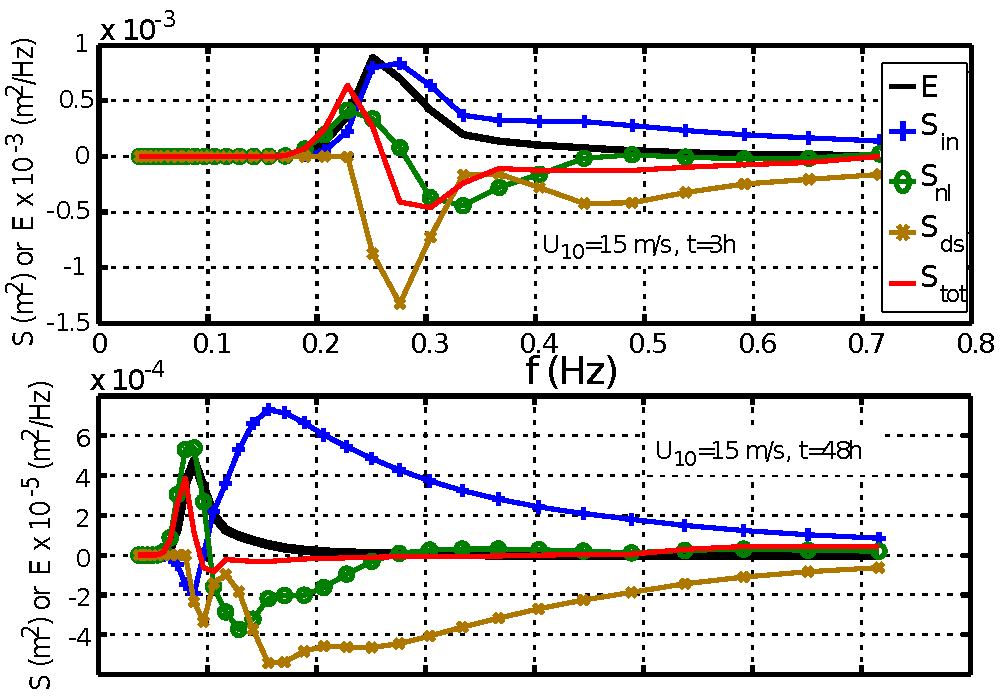
\includegraphics[width=\textwidth]{FIGS_CH_SOURCETERMS/sourcetermsbalance_TEST420.pdf}}
%\vspace{3.64in}
\caption{Source term balance}{Source terms for a wind speed of 15 m/s with a uniform sea starting from rest at $t=0$.
(a) spectrum and source terms after 3 hours, (b) after 2 days.} \label{fig_sourceterms}
\end{figure}

Among the three source terms, $S_{\mathrm{in}}$ defines the range of frequencies where the 
wind sea is generated, with phase speeds less than the wind speed, this is why 
it requires very strong winds to produce long waves that will radiate as swells. At low frequencies $S_{\mathrm{in}}$ is weakly negative.
The energy provided by the wind via $S_{\mathrm{in}}$ is redistributed 
by the wave interaction term $S_{\mathrm{nl}}$ with a flux to both high and low frequencies. The low 
frequency flux makes it possible to have fully developed waves that actually travel faster than the wind, 
with  a peak frequency up to 1.2 times $U_{10}$. The dissipation term $S_{\mathrm{ds}}$ removes the excess of energy 
due to strong wave steepness. 

The sum of the three terms gives the trend of the spectral evolution, which, integrated in 
time gives the evolving spectrum, with an example on figure \ref{fig_sourceterms}. All operational wave models use a 
discretization of the energy balance equation (\ref{EulerianEBEdeep}), with finite differences in time. 

Most differences between models, at least for the windsea part of the spectrum, are due to differences in the parametrizations. 
Figure \ref{fig_sourceterms2D} shows and example of different parametrizations.
Todays most accurate model results have been obtained with the parametrizations by \cite{Rascle&Ardhuin2013}. There are still problems 
at short fetch and for high frequencies, with a poor representation of the directional distribution and an overestimation of the energy 
level at $f > 3 f_p$. This is why the parameterization by \cite{Romero2019} has been designed to correct some of these shorter wave problems.

%%%%%%%%%%%%%%%%%%%%%%%%%%%%%%%%%%%%%%%%%%%%%%%%%%%%%%%%%%%%%%%%%%%%%%%% figure
\begin{figure}[bht]
\centerline{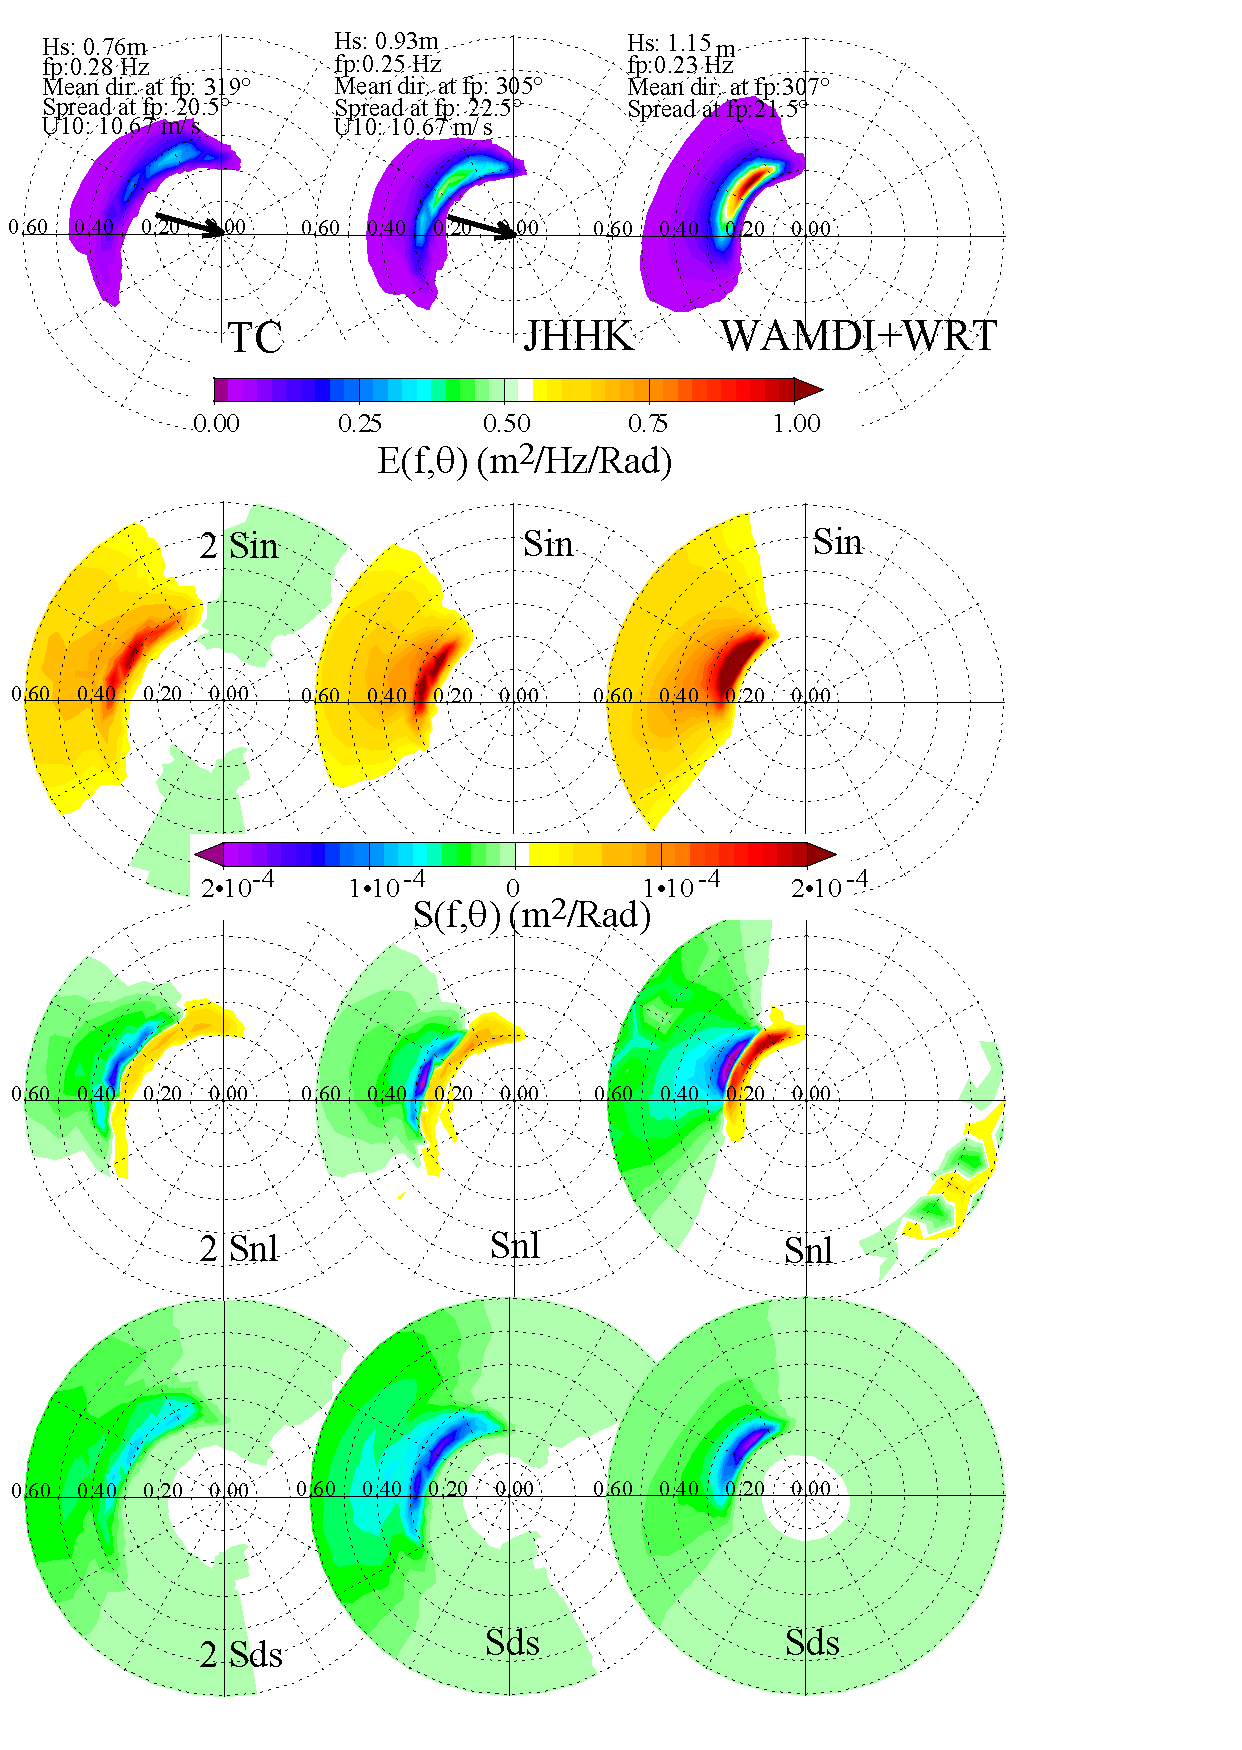
\includegraphics[width=0.6\textwidth]{FIGS_CH_SOURCETERMS/termesource2D.pdf}}
%\vspace{3.64in}
\caption{Three sets of parameterizations, three different balances}{Source terms for a wind speed of 10 m/s at a 
fetch of 40~km. Left: parametrization by \cite{Tolman&Chalikov1996} with much weaker input and disspation,
center:  WAM-Cycle 4 \citep{Janssen&al.1994}, right WAM-Cycle 3 in which the DIA parametrization has been replaced 
by an exact calculation of the interactions. The \cite{Tolman&Chalikov1996} 
terms have been multiplied by 2 in order to be in the same range. Picture from \cite{Ardhuin&al.2007}.}
\label{fig_sourceterms2D}
\end{figure}
%%%%%%%%%%%%%%%%%%%%%%%%%%%%%%%%%%%%%%%%%%%%%%%%%%%%%%%%%%%%%%%%%%%%%%%% figure
